%===================================== APPENDIX B =================================
\chapter{User Manual} \label{app:user-manual}

% is missing what happens when clicking the 'Visualizer' link.

\textbf{Note:} This appendix explains how to use the web interface of the visualization tool. Remember that certain parts of the functionality requires that you have added the available callbacks to your Keras network script. We refer the user to appendix \ref{app:callbacks-api} for the callbacks API, as well as an explanation of how to use them in a script. \\

\noindent The web interface is fairly simple to use. At all times, the top of the page will show a navigation bar with links to the available pages. When clicked, these links take you to the corresponding page. The interface will display error feedback for any illegal action you might take, such as trying to log in with a mismatching username and password, or trying to upload a file with a filename that is not unique. Similarly, feedback for successful activity, like uploading a file, is also shown. \\

% Login page

\begin{figure}[h!]
    \centering
        \frame{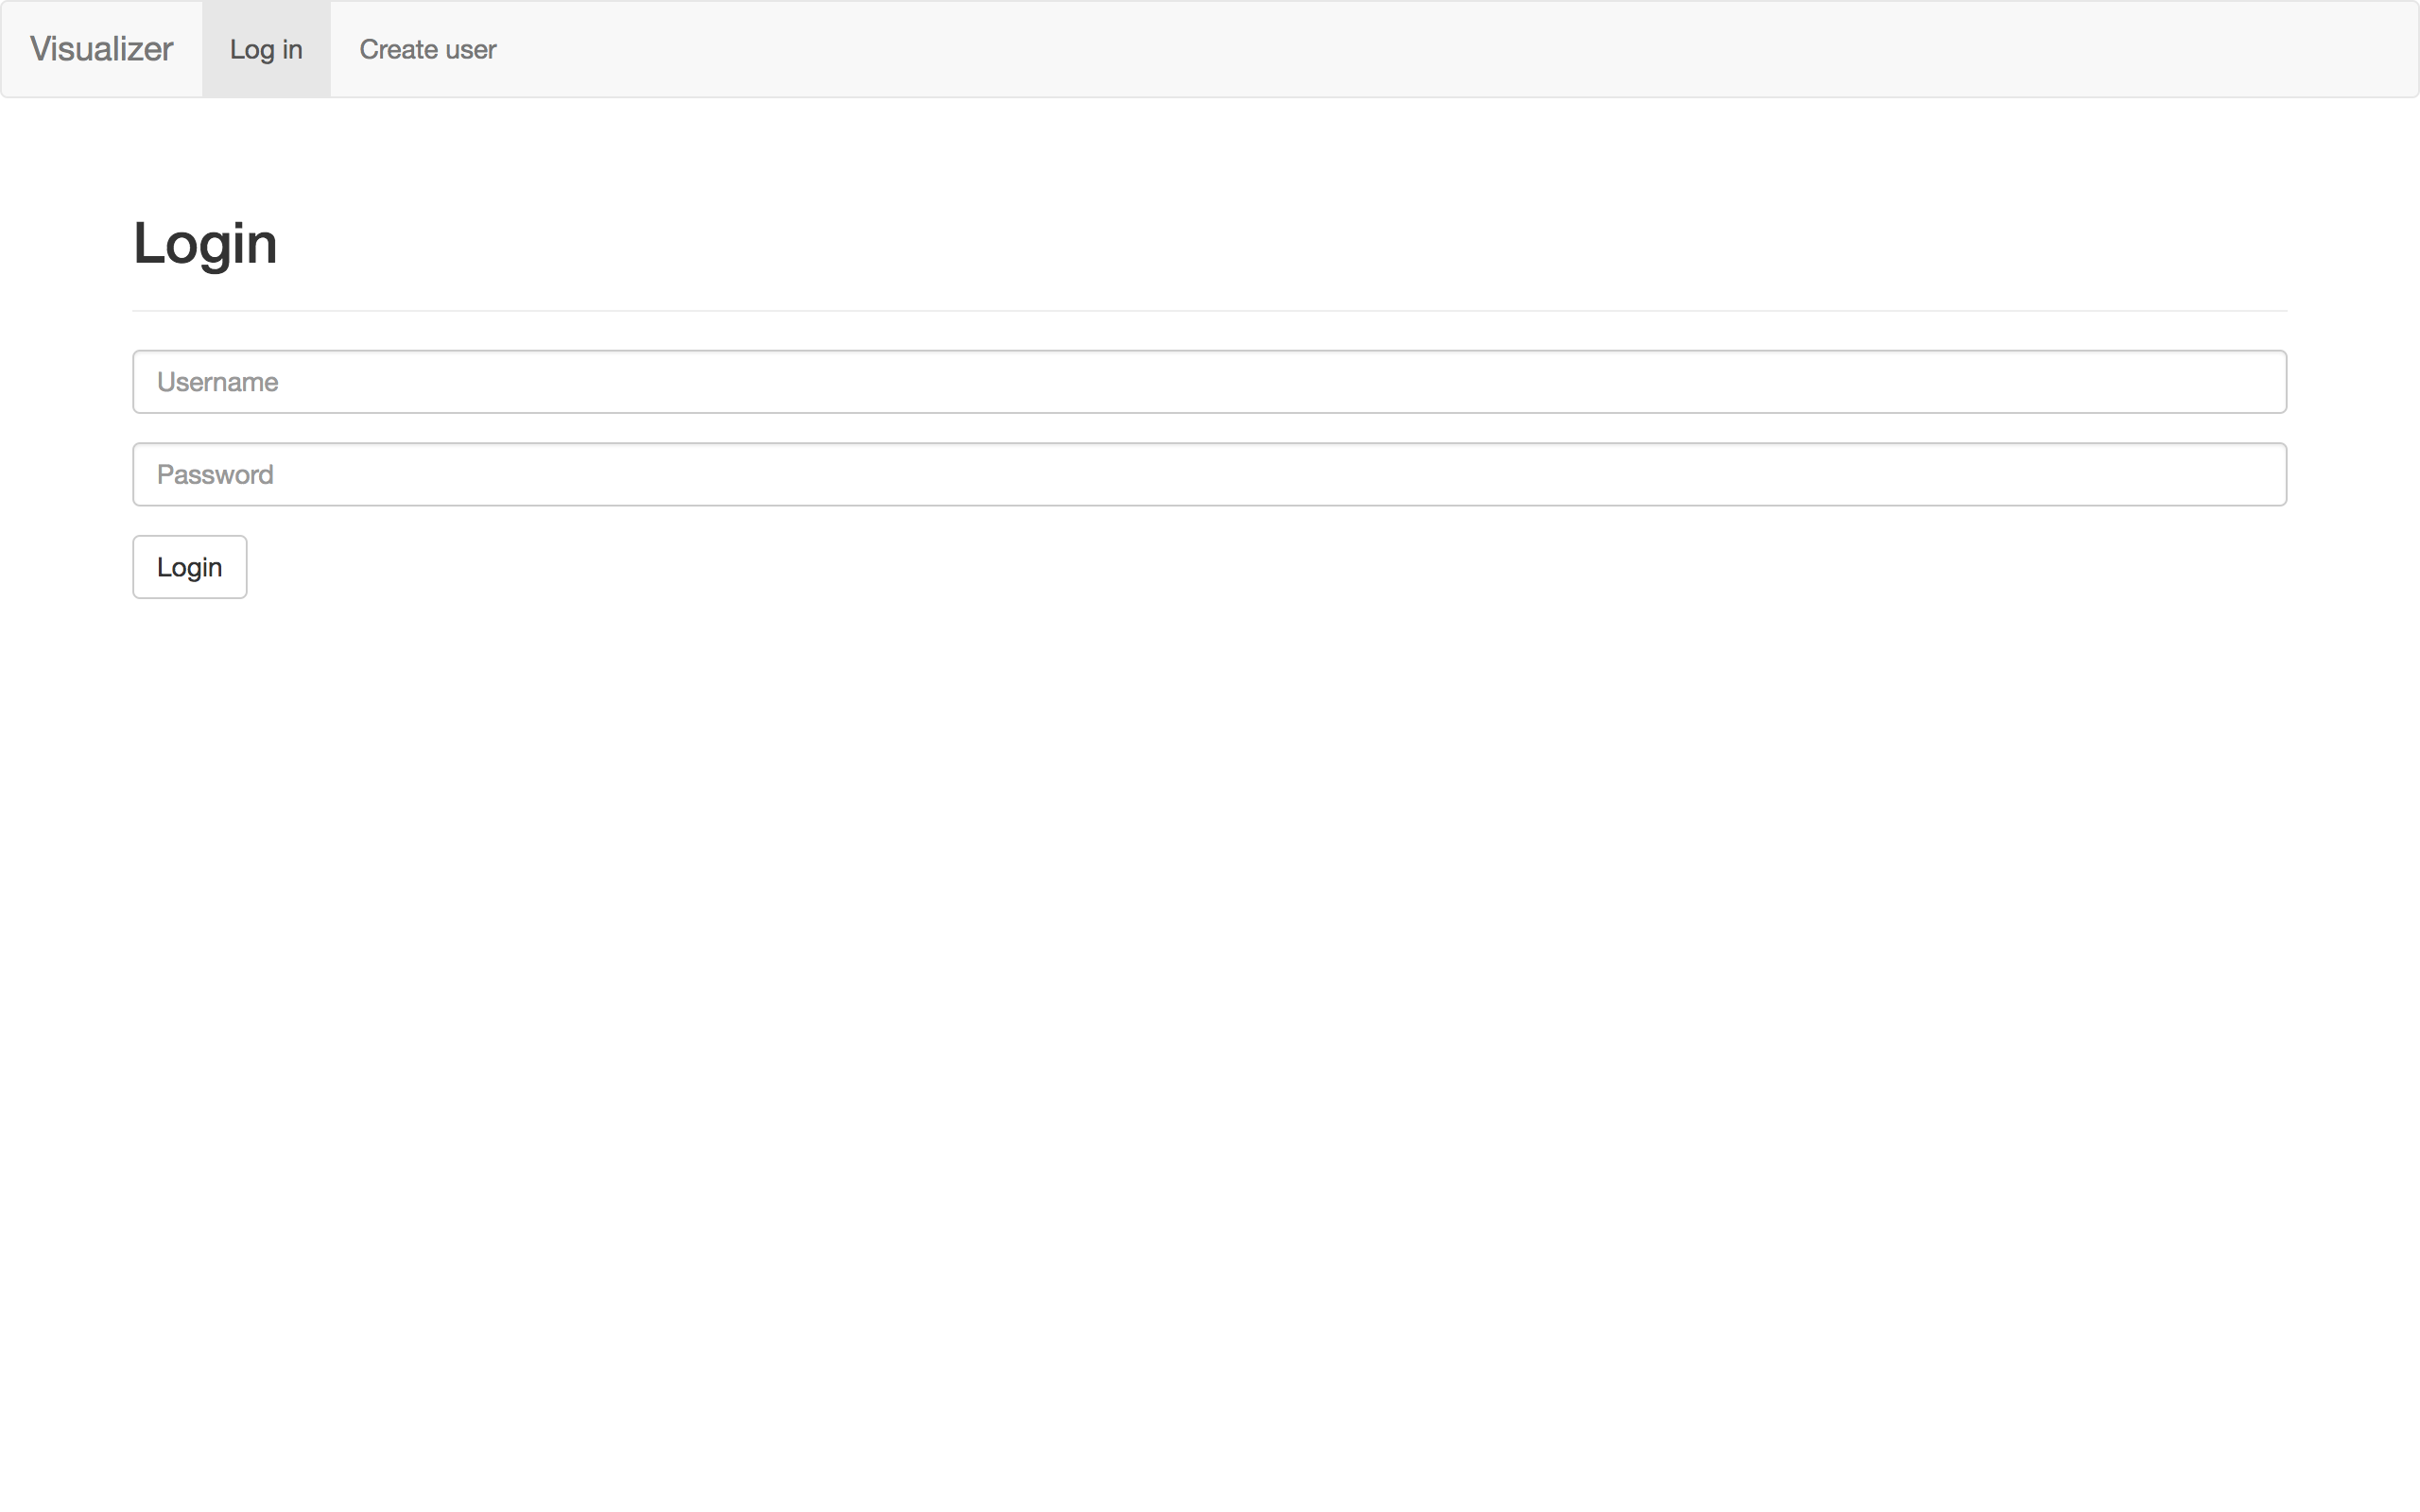
\includegraphics[width=0.8\textwidth]{fig/screenshots/login.png}}
        \caption{Login}
        \label{login}
\end{figure}

% create user

\begin{figure}[h!]
    \centering
        \frame{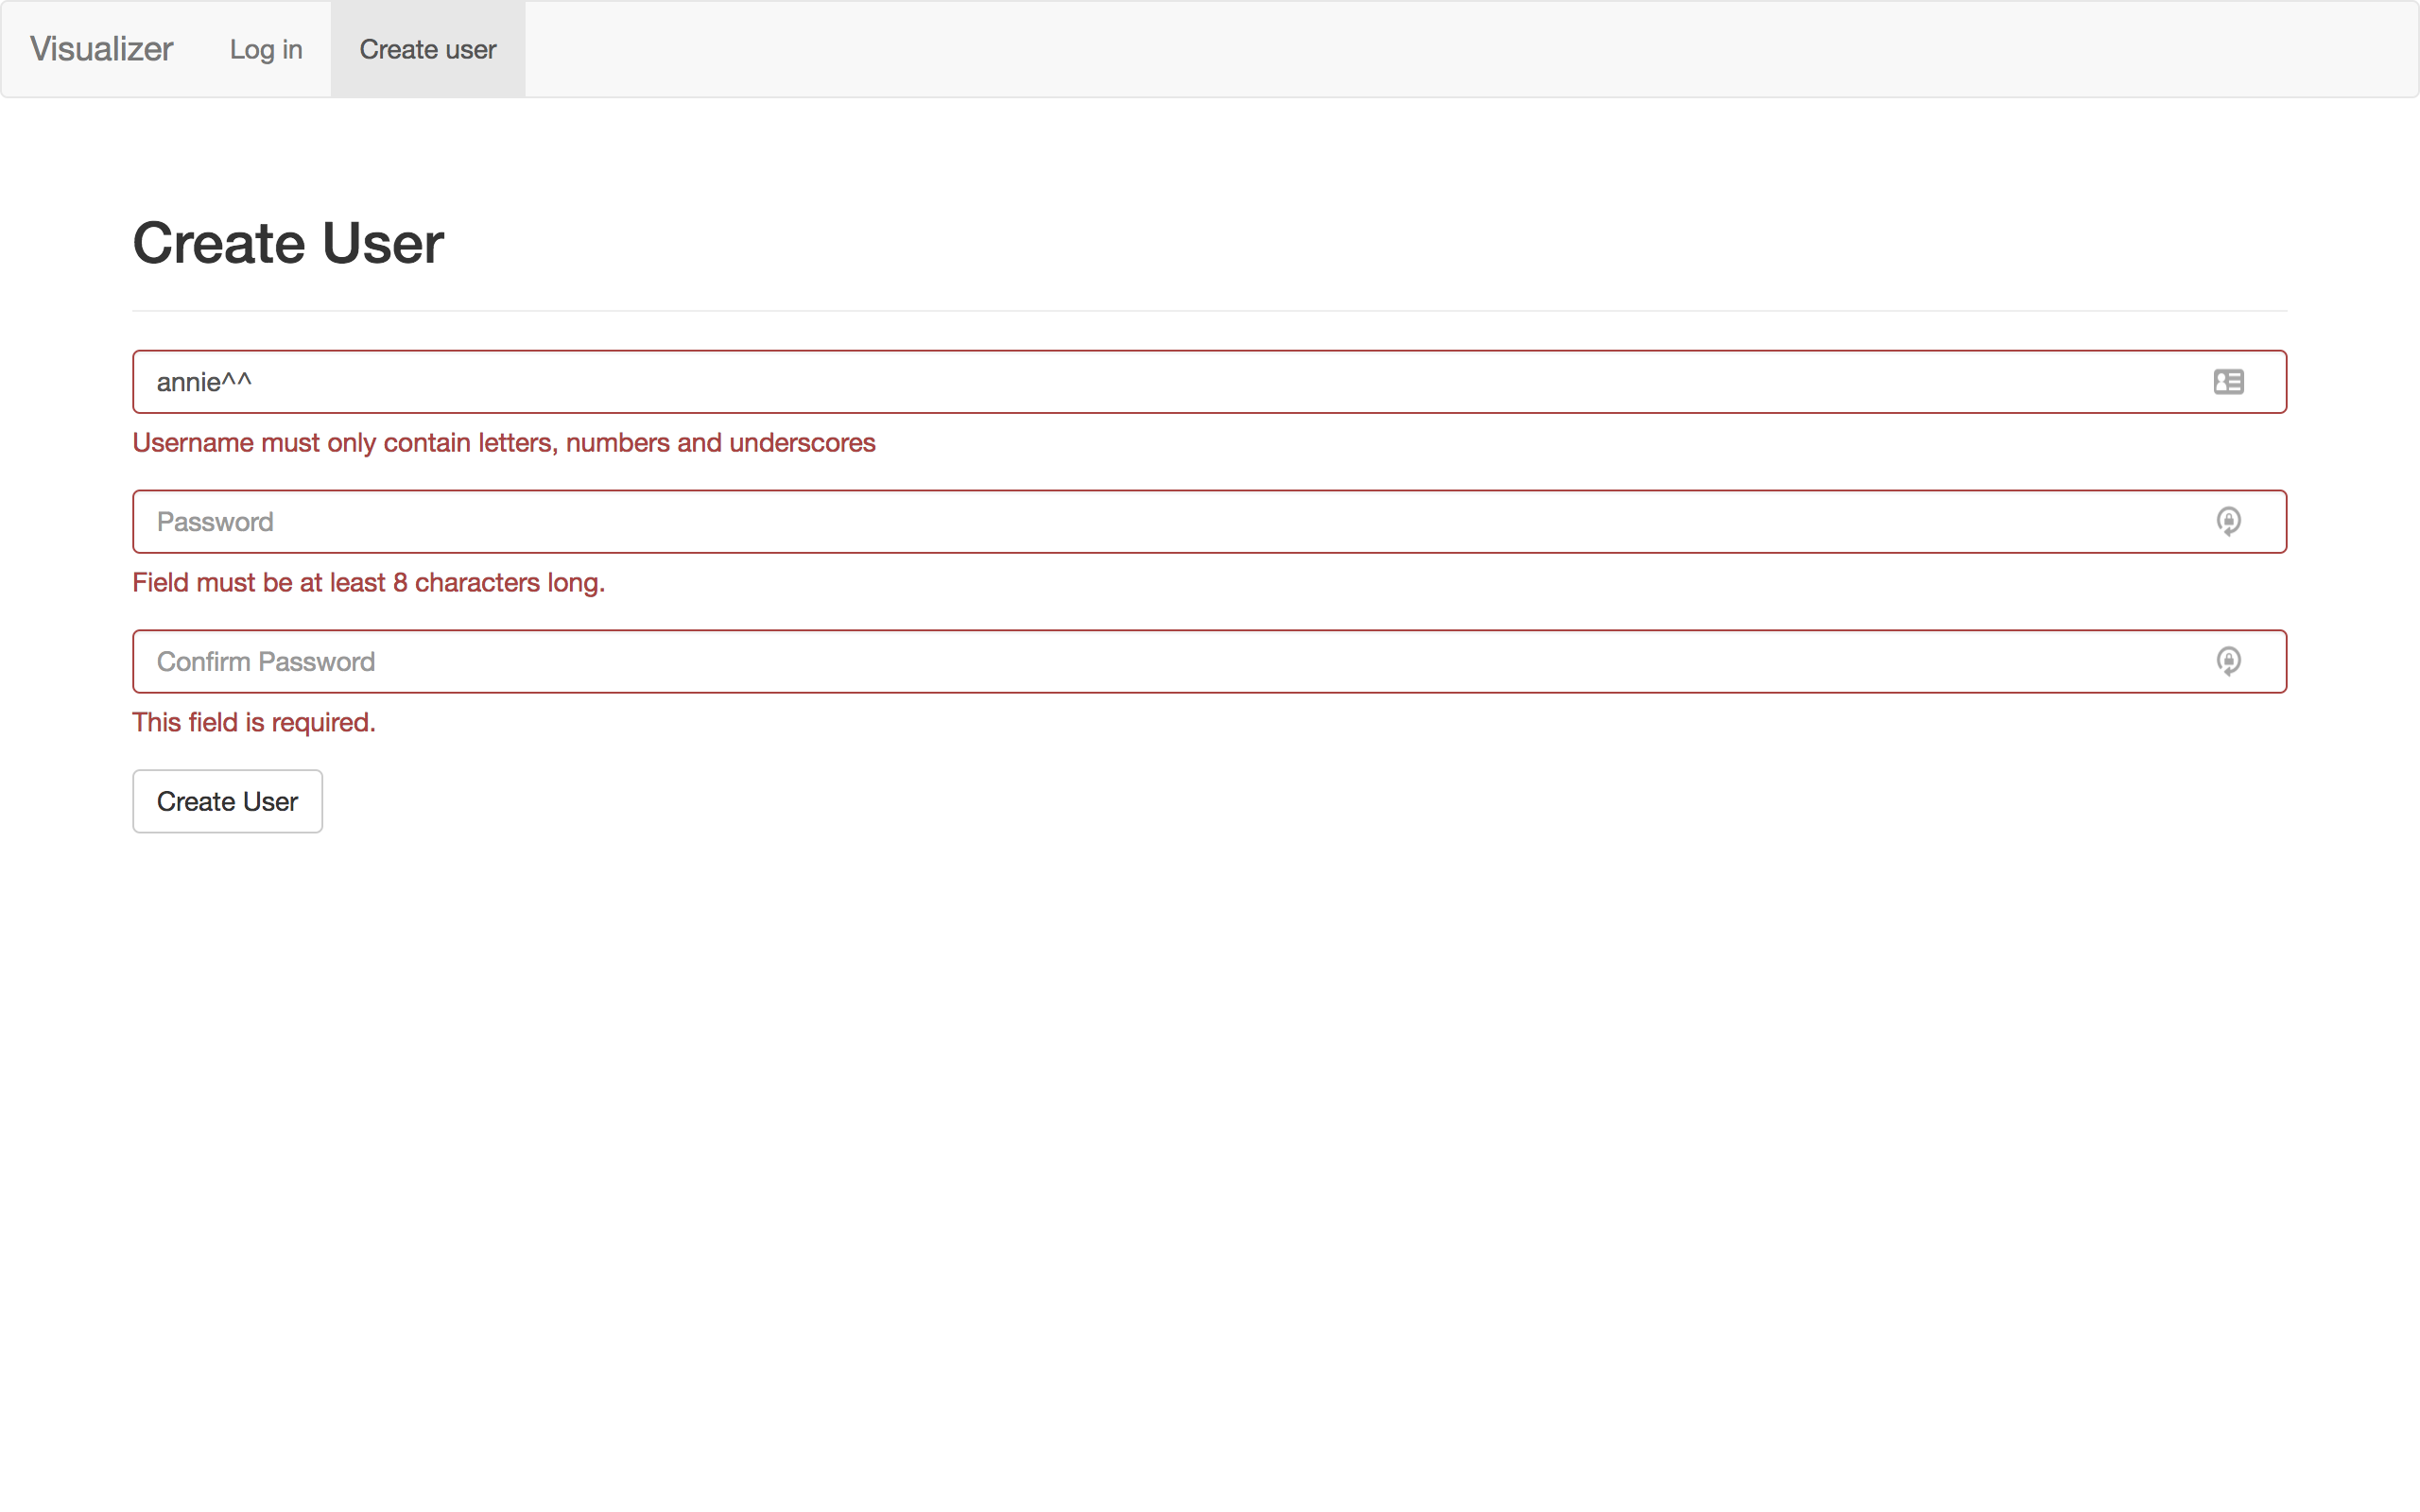
\includegraphics[width=0.8\textwidth]{fig/screenshots/create_user_error.png}}
        \caption{Creating a new user}
        \label{create-user}
\end{figure}

\noindent When starting the visualization tool, you will be shown a login page as in \textbf{Fig. \ref{login}}. If you do not already have a user, you can click the "Create user" link to create a new user for the application. Usernames must be between 5 and 20 characters long, and can only contain alphanumerical characters and underscores. The username must also be unique. The password must be minimum 8 characters and can only contain alphanumeric characters. As seen in \textbf{Fig. \ref{create-user}}, the interface will provide you with descriptive feedback if any of these restrictions are broken. When you have successfully created a user, you are automatically redirected back to the login page, where you can log in to start using the visualization tool. \\

% Uploaded files

\begin{figure}[h!]
    \centering
        \frame{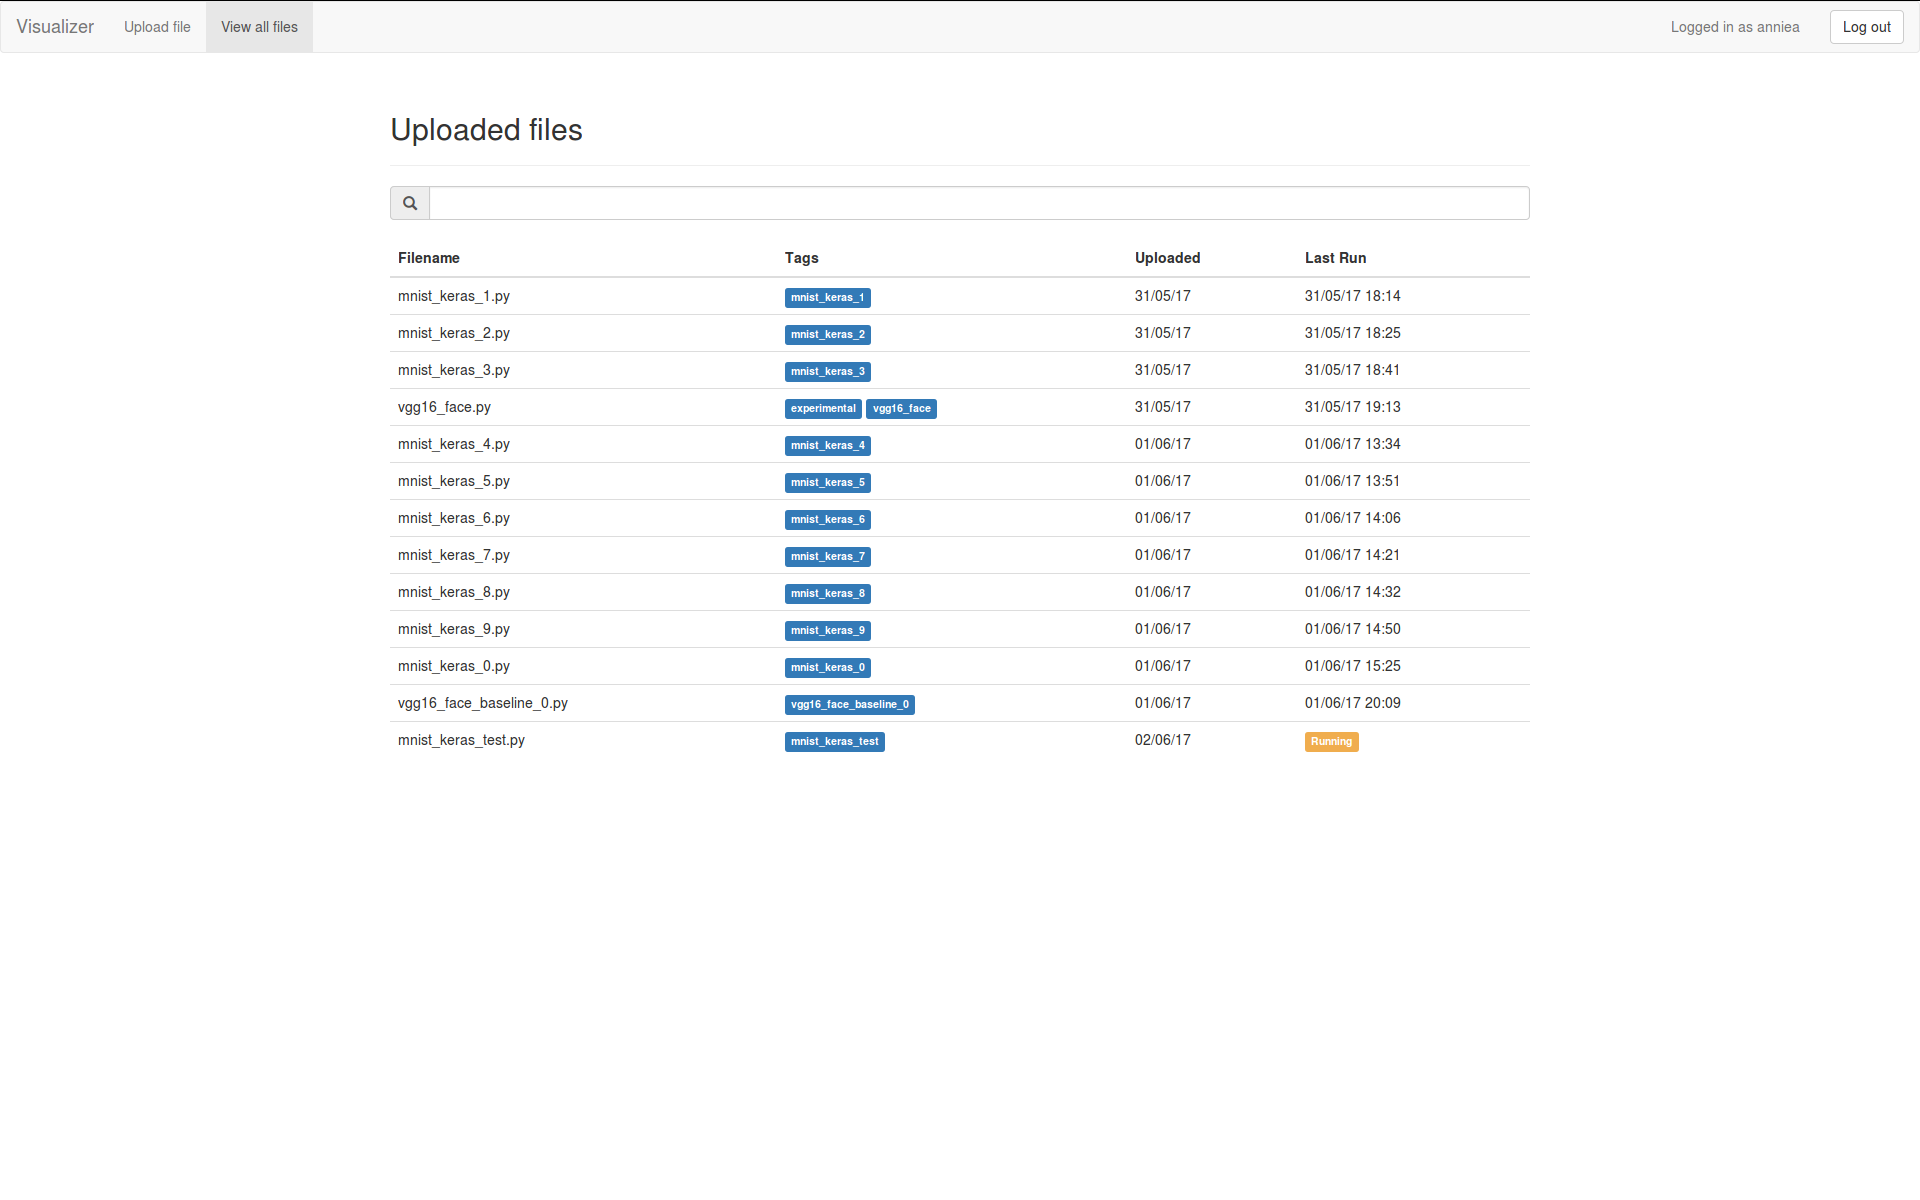
\includegraphics[width=0.8\textwidth]{fig/screenshots_old/all_files_many.png}}
        \caption{Uploaded files}
        \label{all-files}
\end{figure}

\noindent When you have logged in, you will be directed to the page in \textbf{Fig. \ref{all-files}} showing all your uploaded files. If there are no uploaded files yet, the page will suggest that you click on a link to upload a file. If you already have files uploaded, these will be displayed in a list with columns containing the filename, tags, upload date, and the date that the file was last ran. If the file is currently running, the last column will show a yellow label that reads "Running". You can sort the list by clicking on the various columns. A search bar is also provided, and it responds to filenames and tags. Clicking on an entry in the list will take you to the corresponding file's overview page. First, we will describe the upload page. \\

% upload file

\begin{figure}[h!]
    \centering
        \frame{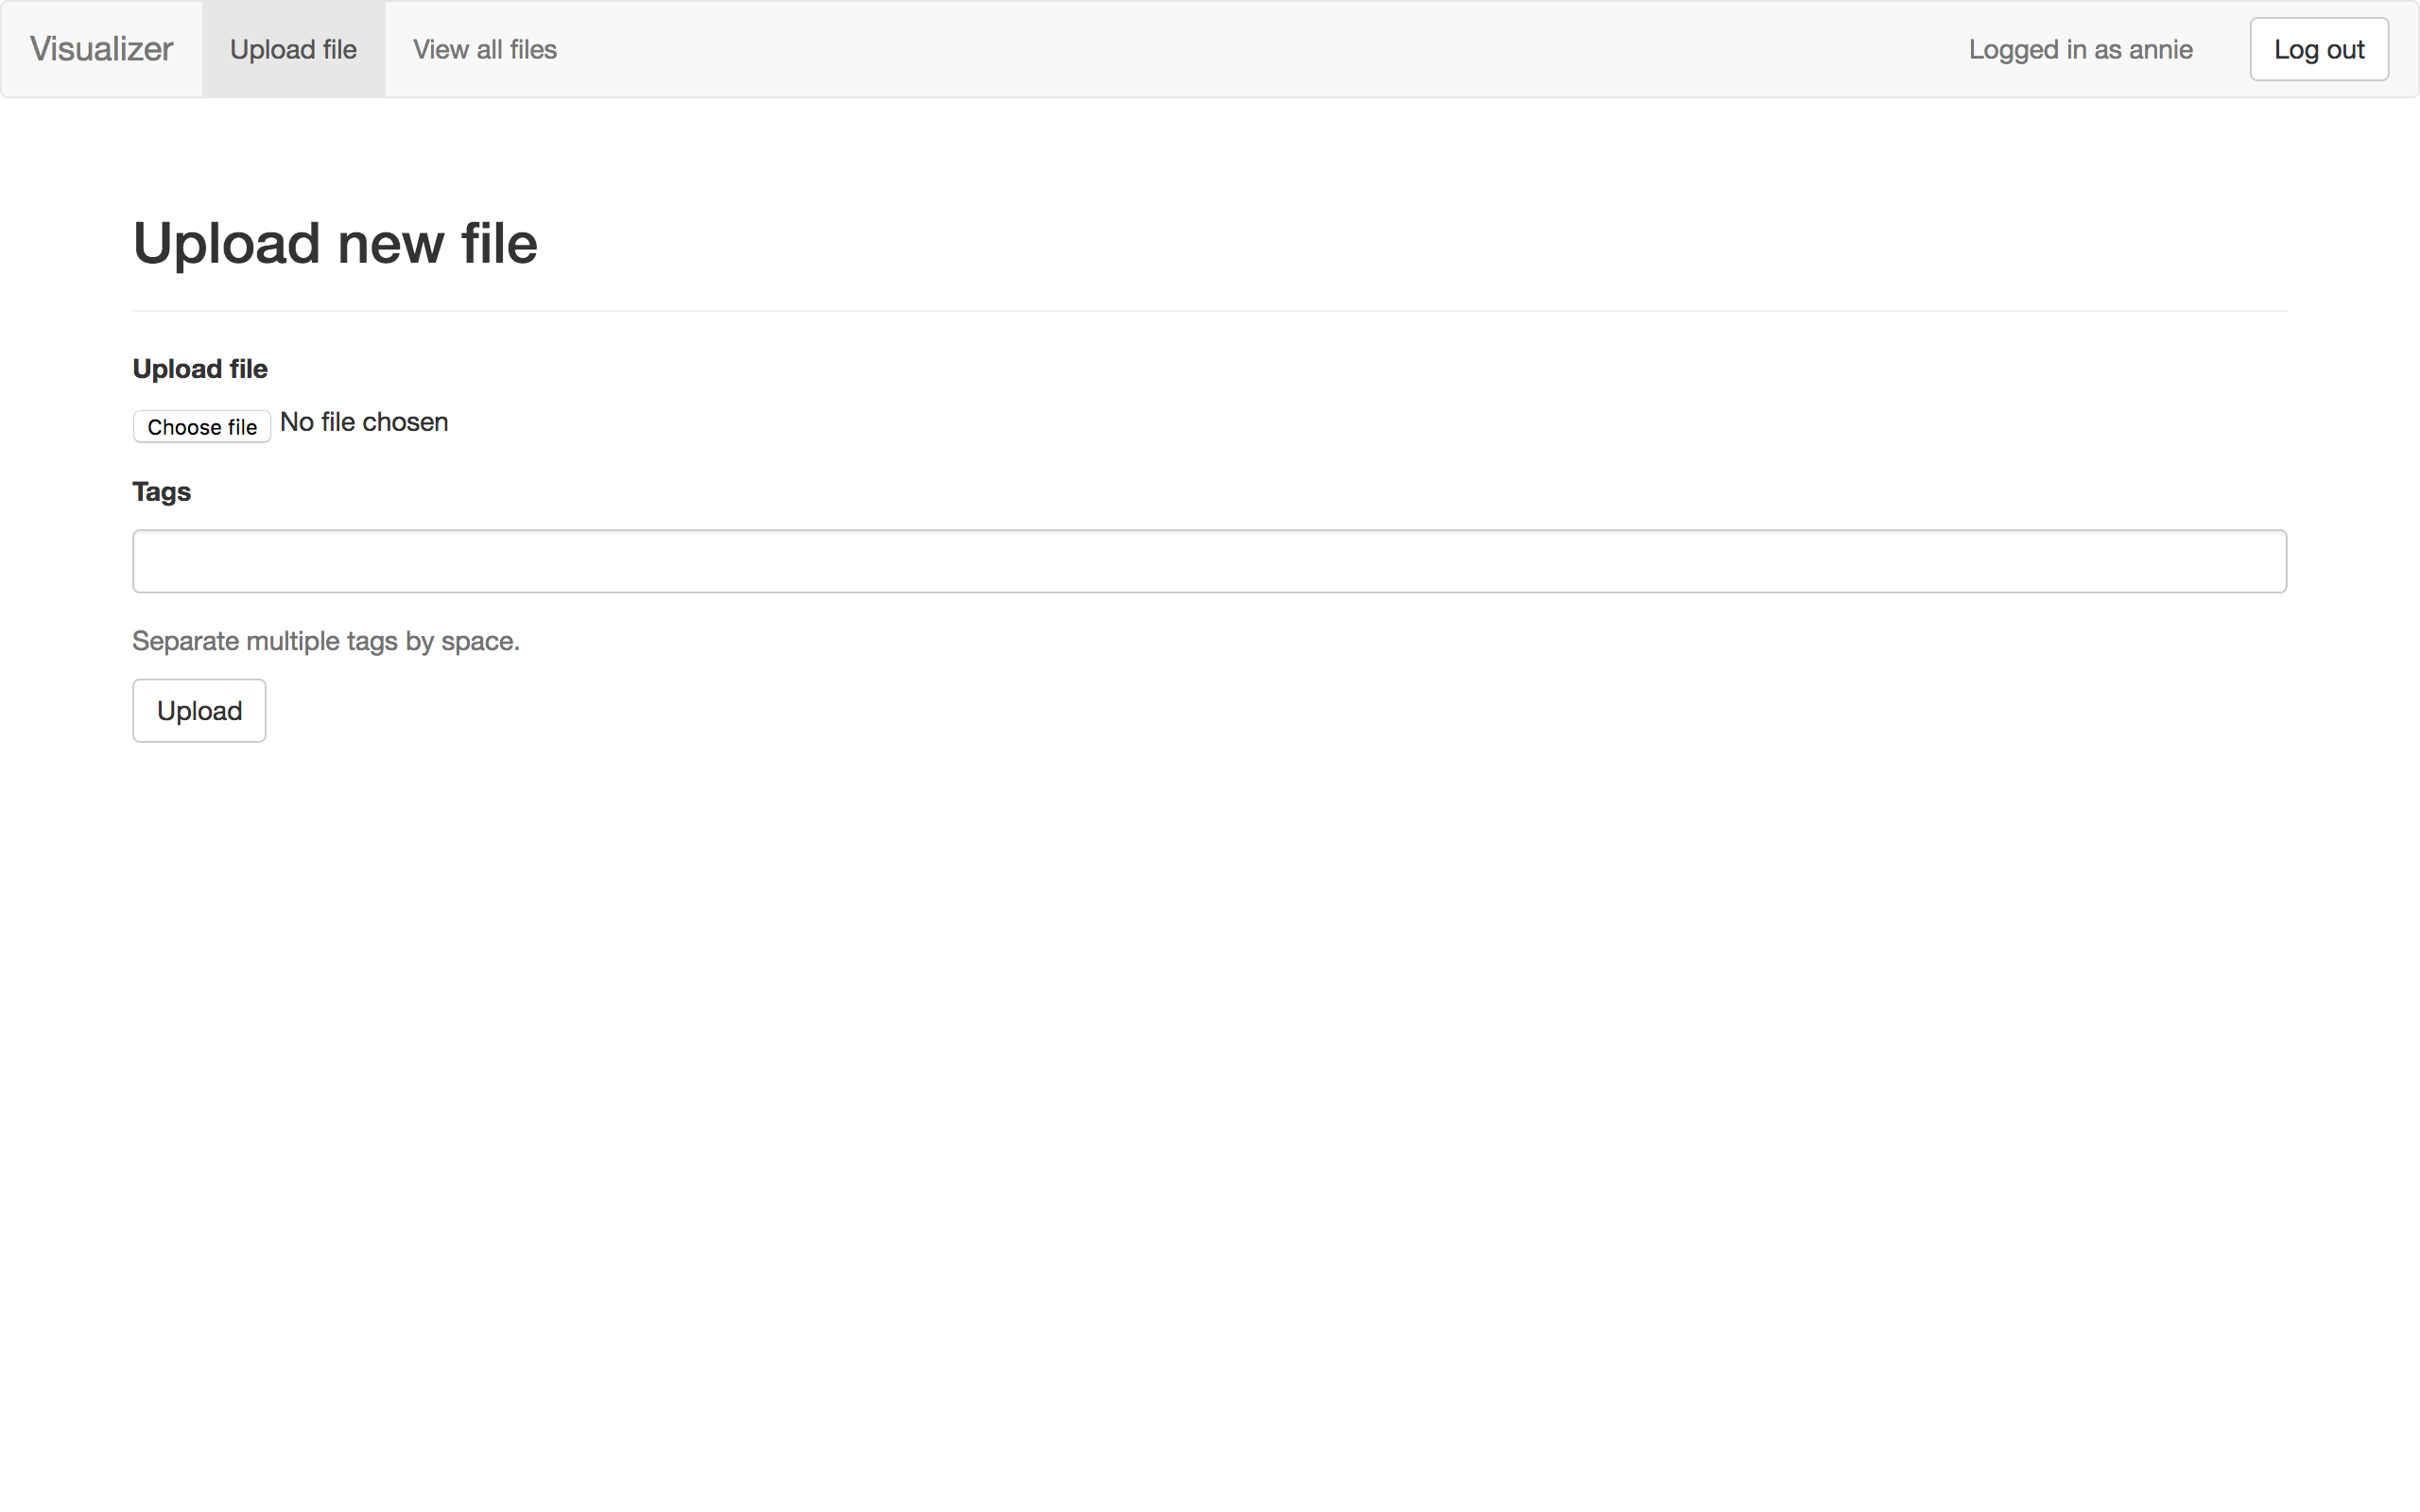
\includegraphics[width=0.8\textwidth]{fig/screenshots/upload_file.png}}
        \caption{Uploading a file}
        \label{upload-file}
\end{figure}

\noindent You can upload Keras network scripts from your computer on the file upload page, as seen in \textbf{Fig. \ref{upload-file}}. The file uploaded will retain its filename, which must be unique. To better organize your files, you can associate tags to the file before uploading. The tags are split at whitespaces, for instance 'neural network' will result in two tags: "neural" and "network". Use underscores if you want to add tags containing multiple words. The filename, without its extension, will be automatically added as a tag. \\

\begin{figure}[h!]
    \centering
        \frame{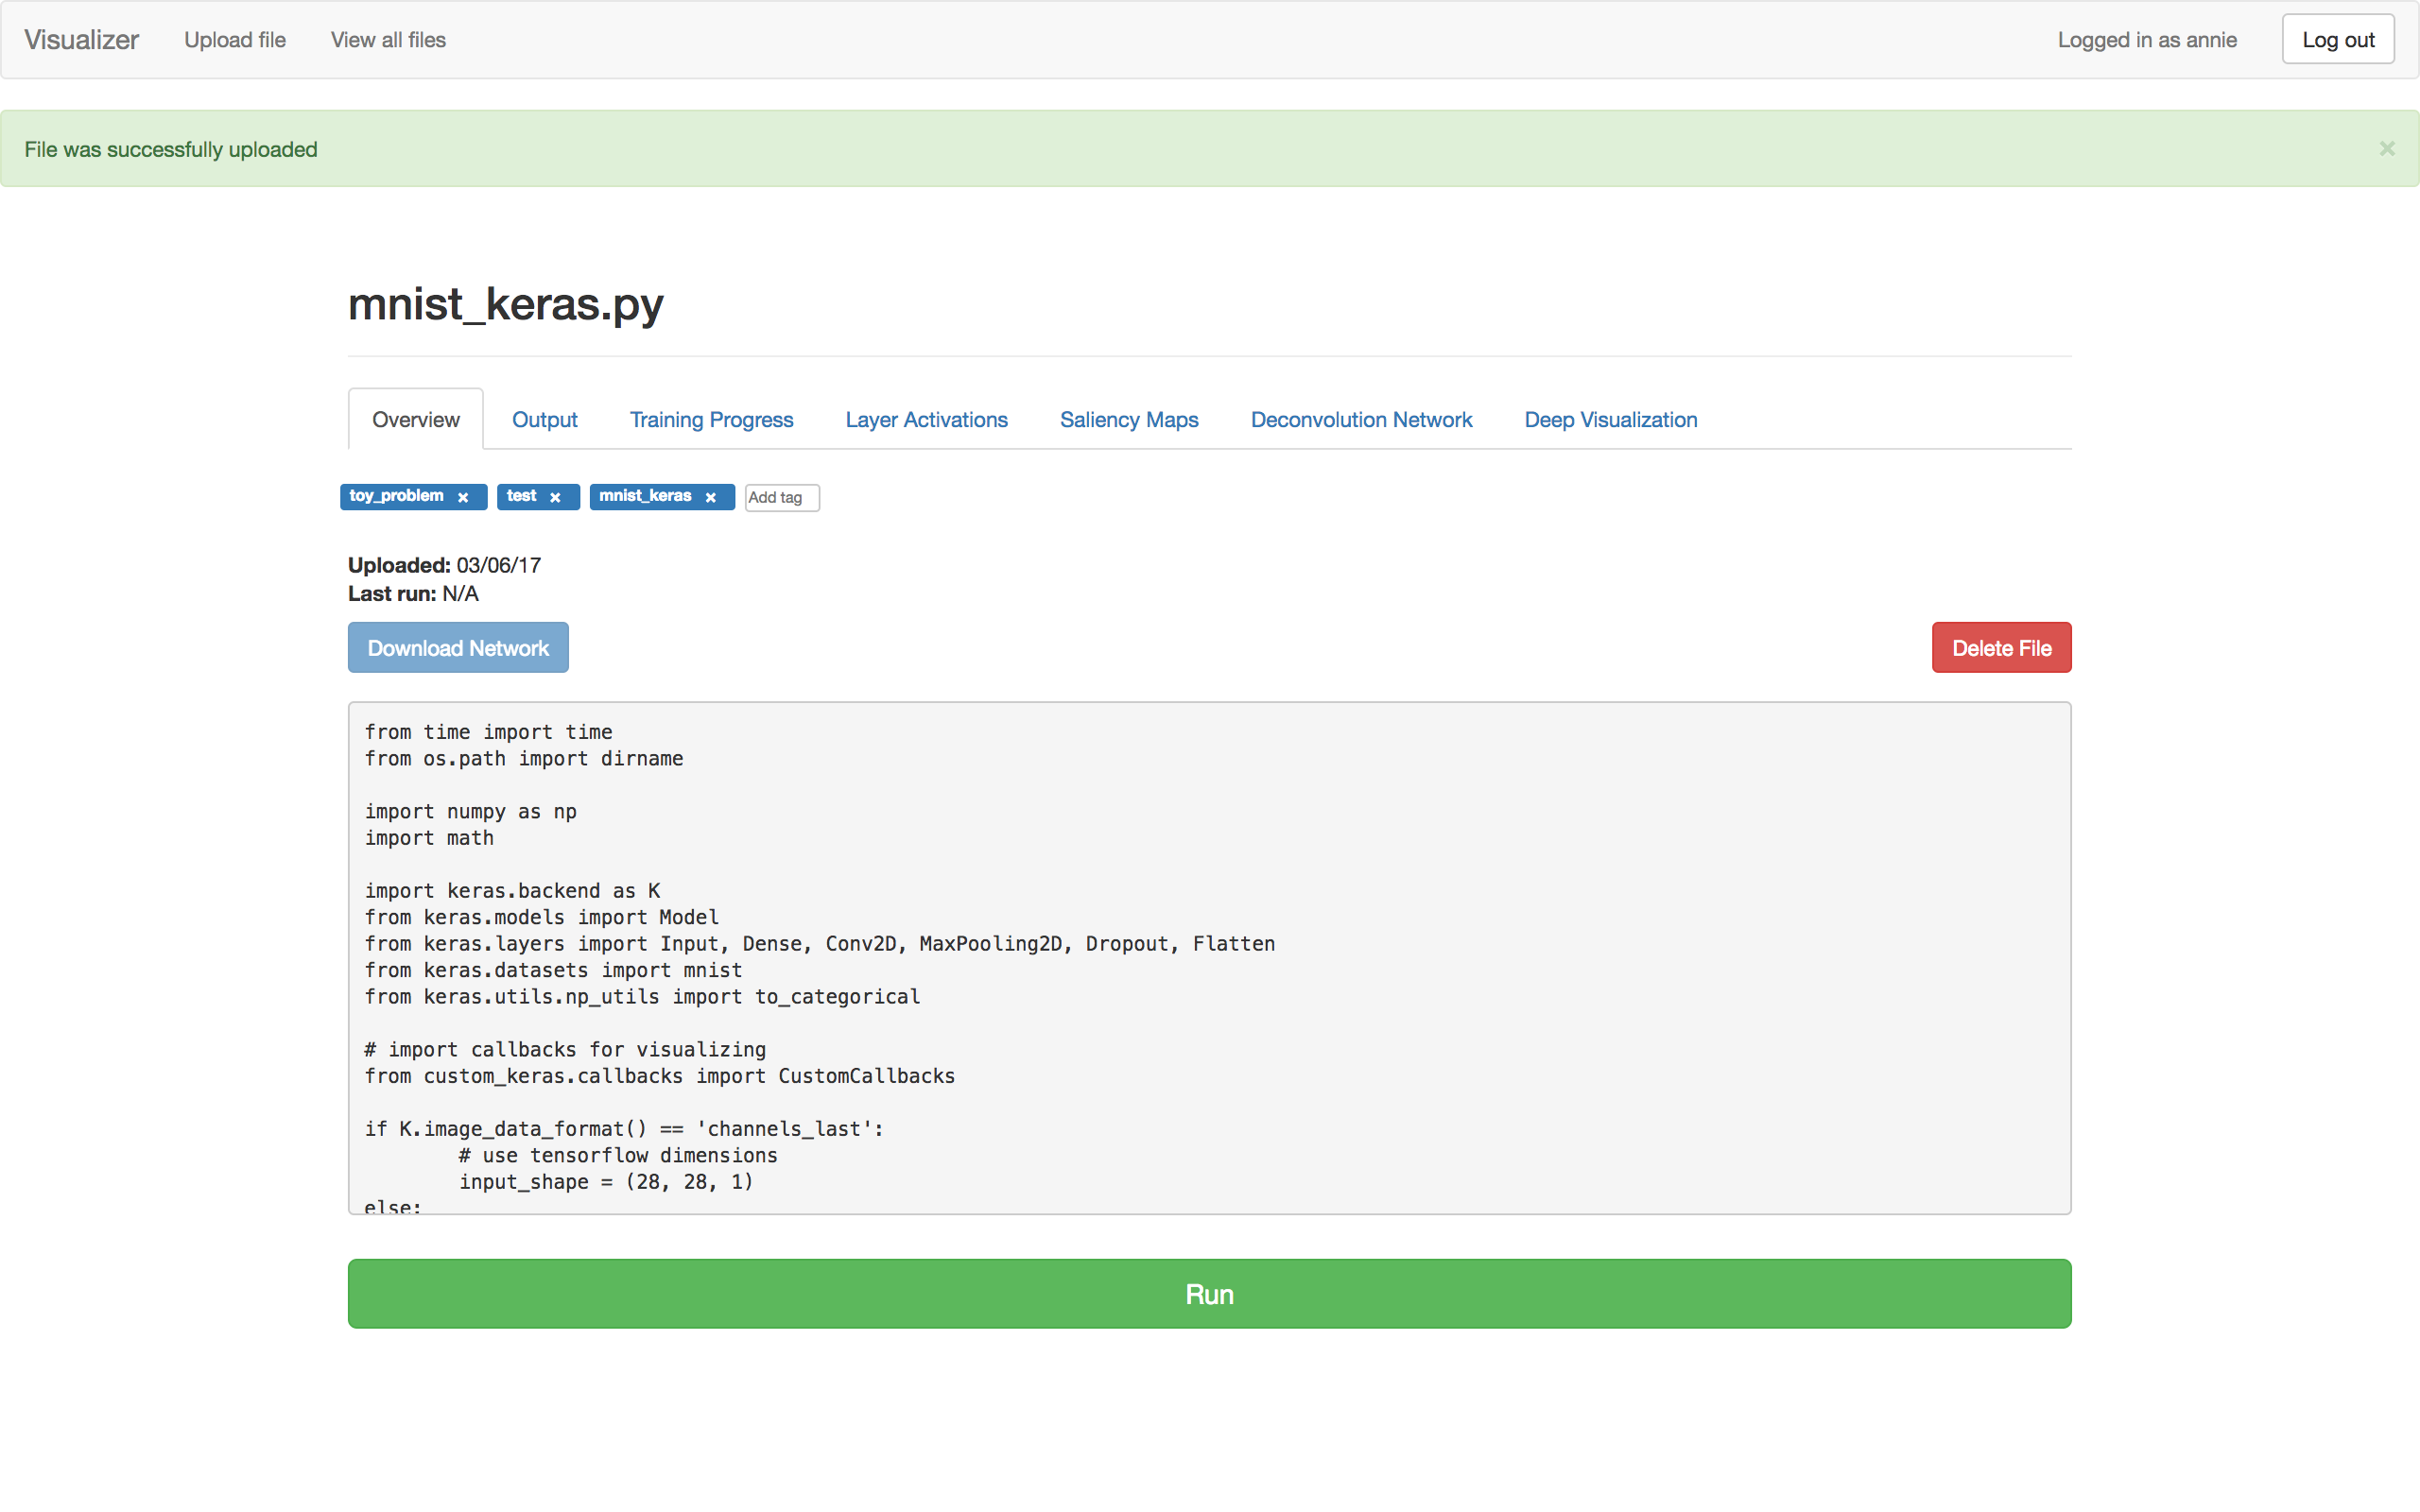
\includegraphics[width=0.8\textwidth]{fig/screenshots/file_uploaded.png}}
        \caption{File overview}
        \label{file-overview}
\end{figure}

\begin{figure}[h!]
    \centering
        \frame{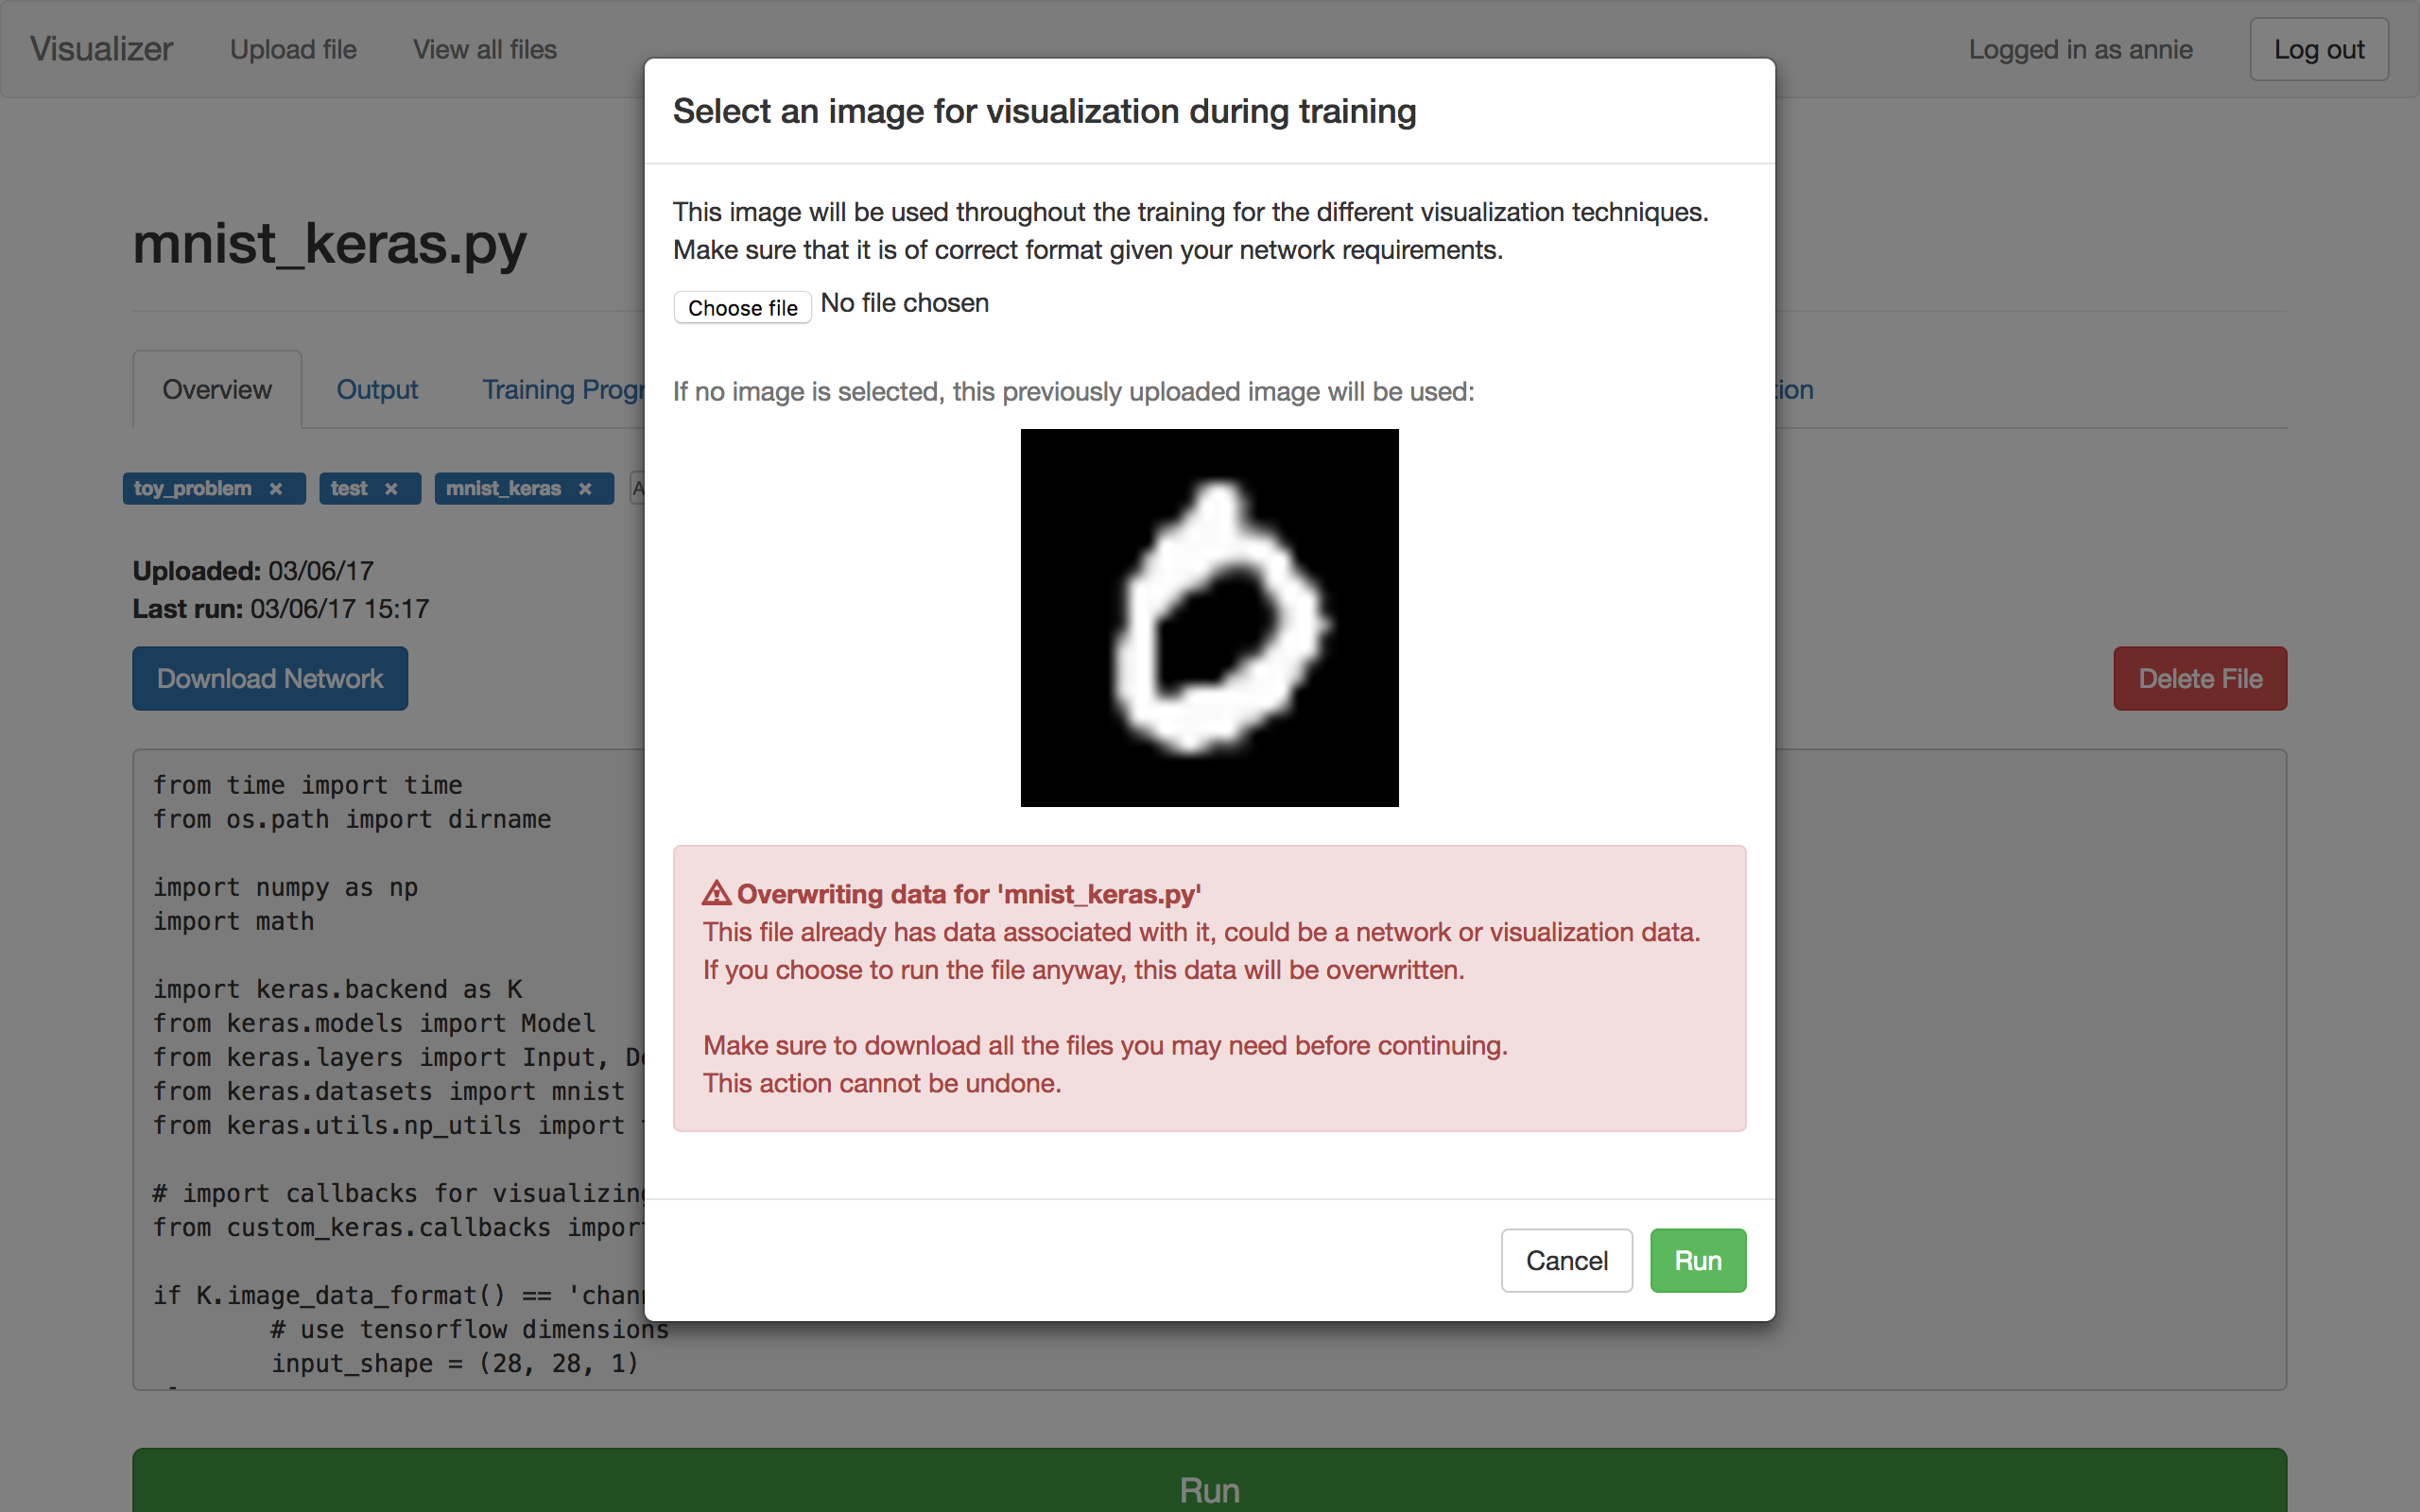
\includegraphics[width=0.8\textwidth]{fig/screenshots/run_file.png}}
        \caption{Running a file}
        \label{run-file}
\end{figure}

\begin{figure}[h!]
    \centering
        \frame{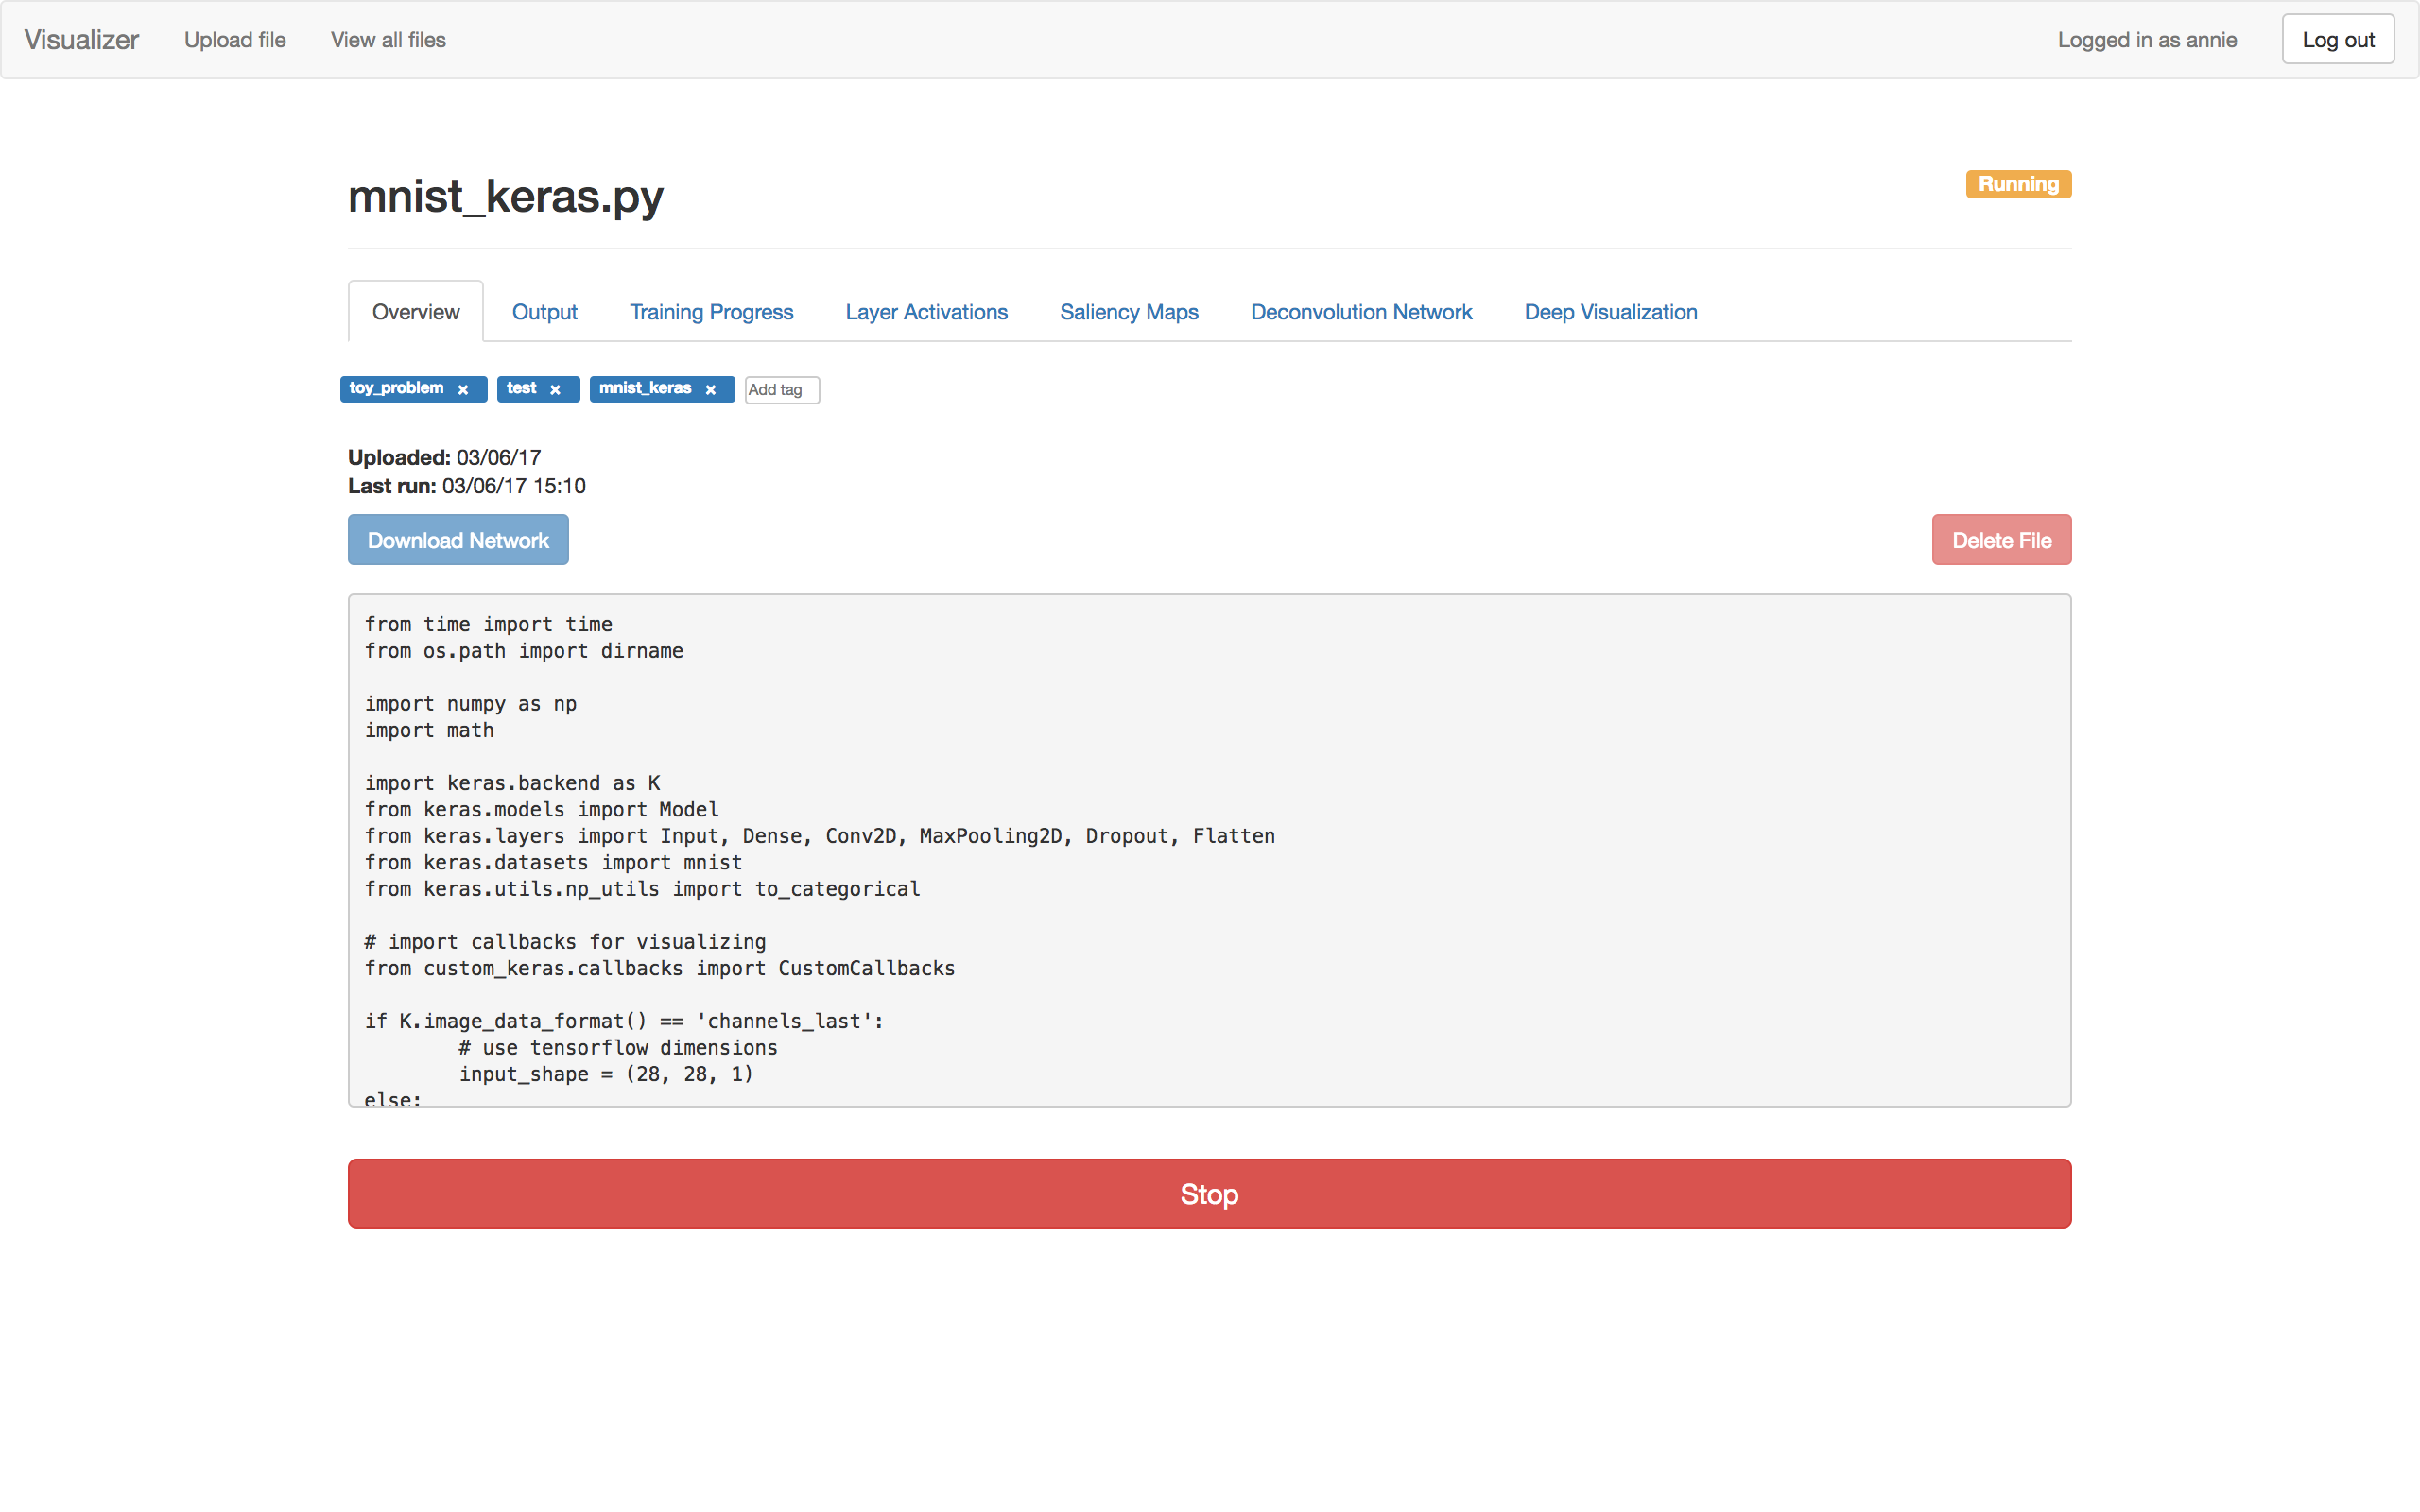
\includegraphics[width=0.8\textwidth]{fig/screenshots/file_running.png}}
        \caption{File overview when file is running}
        \label{file-running}
\end{figure}

\noindent When a file is successfully uploaded, you are taken to the file's overview page, shown in \textbf{Fig. \ref{file-overview}}. A submenu will be available with seven tabs: overview, console output, training progress, layer activations, saliency maps, deconvolutional network and deep visualization. The overview page shows some information about the file, as well as its contents. You have the option of downloading the generated network, assuming that the script includes the network saving callback and has been executed. You can also delete the file if you wish, along with all associated data. Lastly, you can run the file by clicking the green button that reads "Run". Upon clicking the run button, a popup window will appear and ask you to select an image to use for the visualizations. If an image has already been uploaded, that image will be available as a default, as seen in \textbf{Fig. \ref{run-file}}. Upload a new one, or use the previous image and click "Run". Also note that if the file already has been run, it will have data associated with it, for instance networks or visualization data files. Running the file again will delete all of the previously generated data, which the popup warns about. When the popup run button is clicked, the code in the file will be executed in a Python subprocess. When a file is running, it will have the yellow "Running" label displayed at the top right of its page. You can also end the execution of the file at any time by clicking the stop button. A banner with a link to the file will be shown whenever one of your files completes its execution.\\

% output tab

\begin{figure}[h!]
    \centering
        \frame{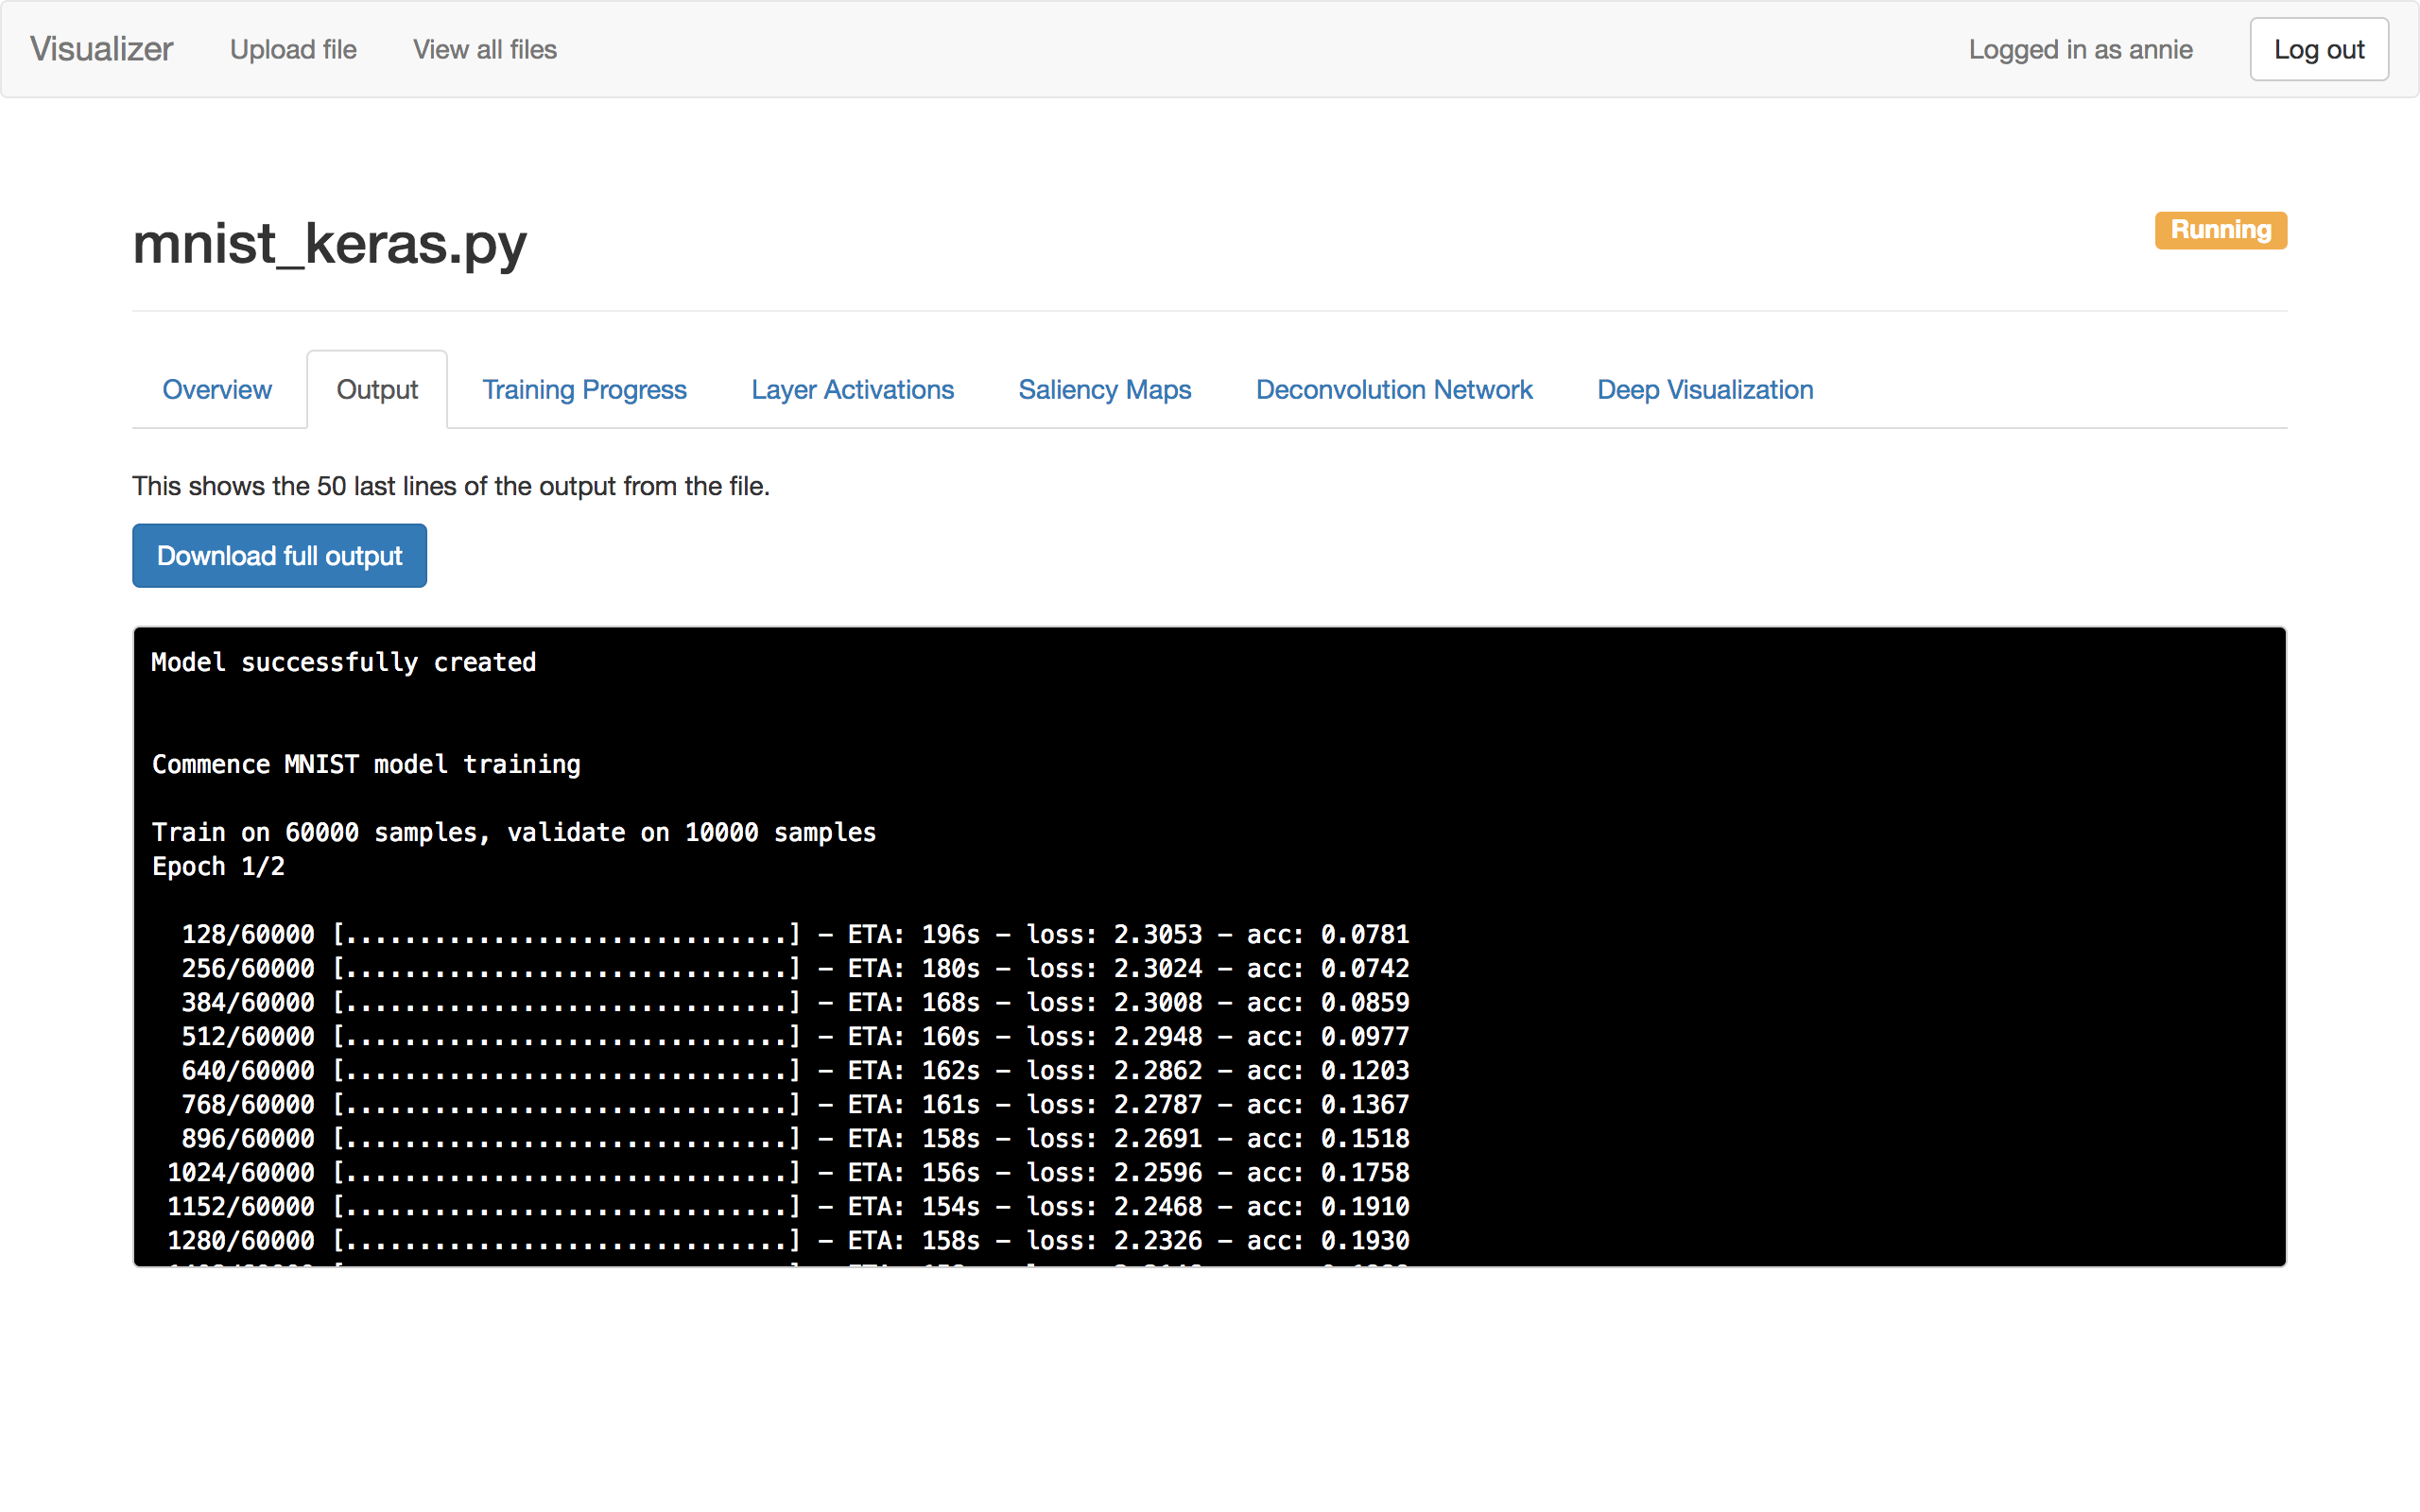
\includegraphics[width=0.8\textwidth]{fig/screenshots/output.png}}
        \caption{Output of a running file}
        \label{output-tab}
\end{figure}

\noindent While a file is running, you can navigate to the various tabs to see different output and visualizations. The output tab in \textbf{Fig. \ref{output-tab}} shows the last 50 lines of the command line output of the file in real-time. The output is useful for viewing estimated time to training completion and epoch accuracy, as well as debugging unexpected halts in the execution. You can download the full output by clicking the button. \\

% Training progress val

\begin{figure}[h!]
    \centering
        \frame{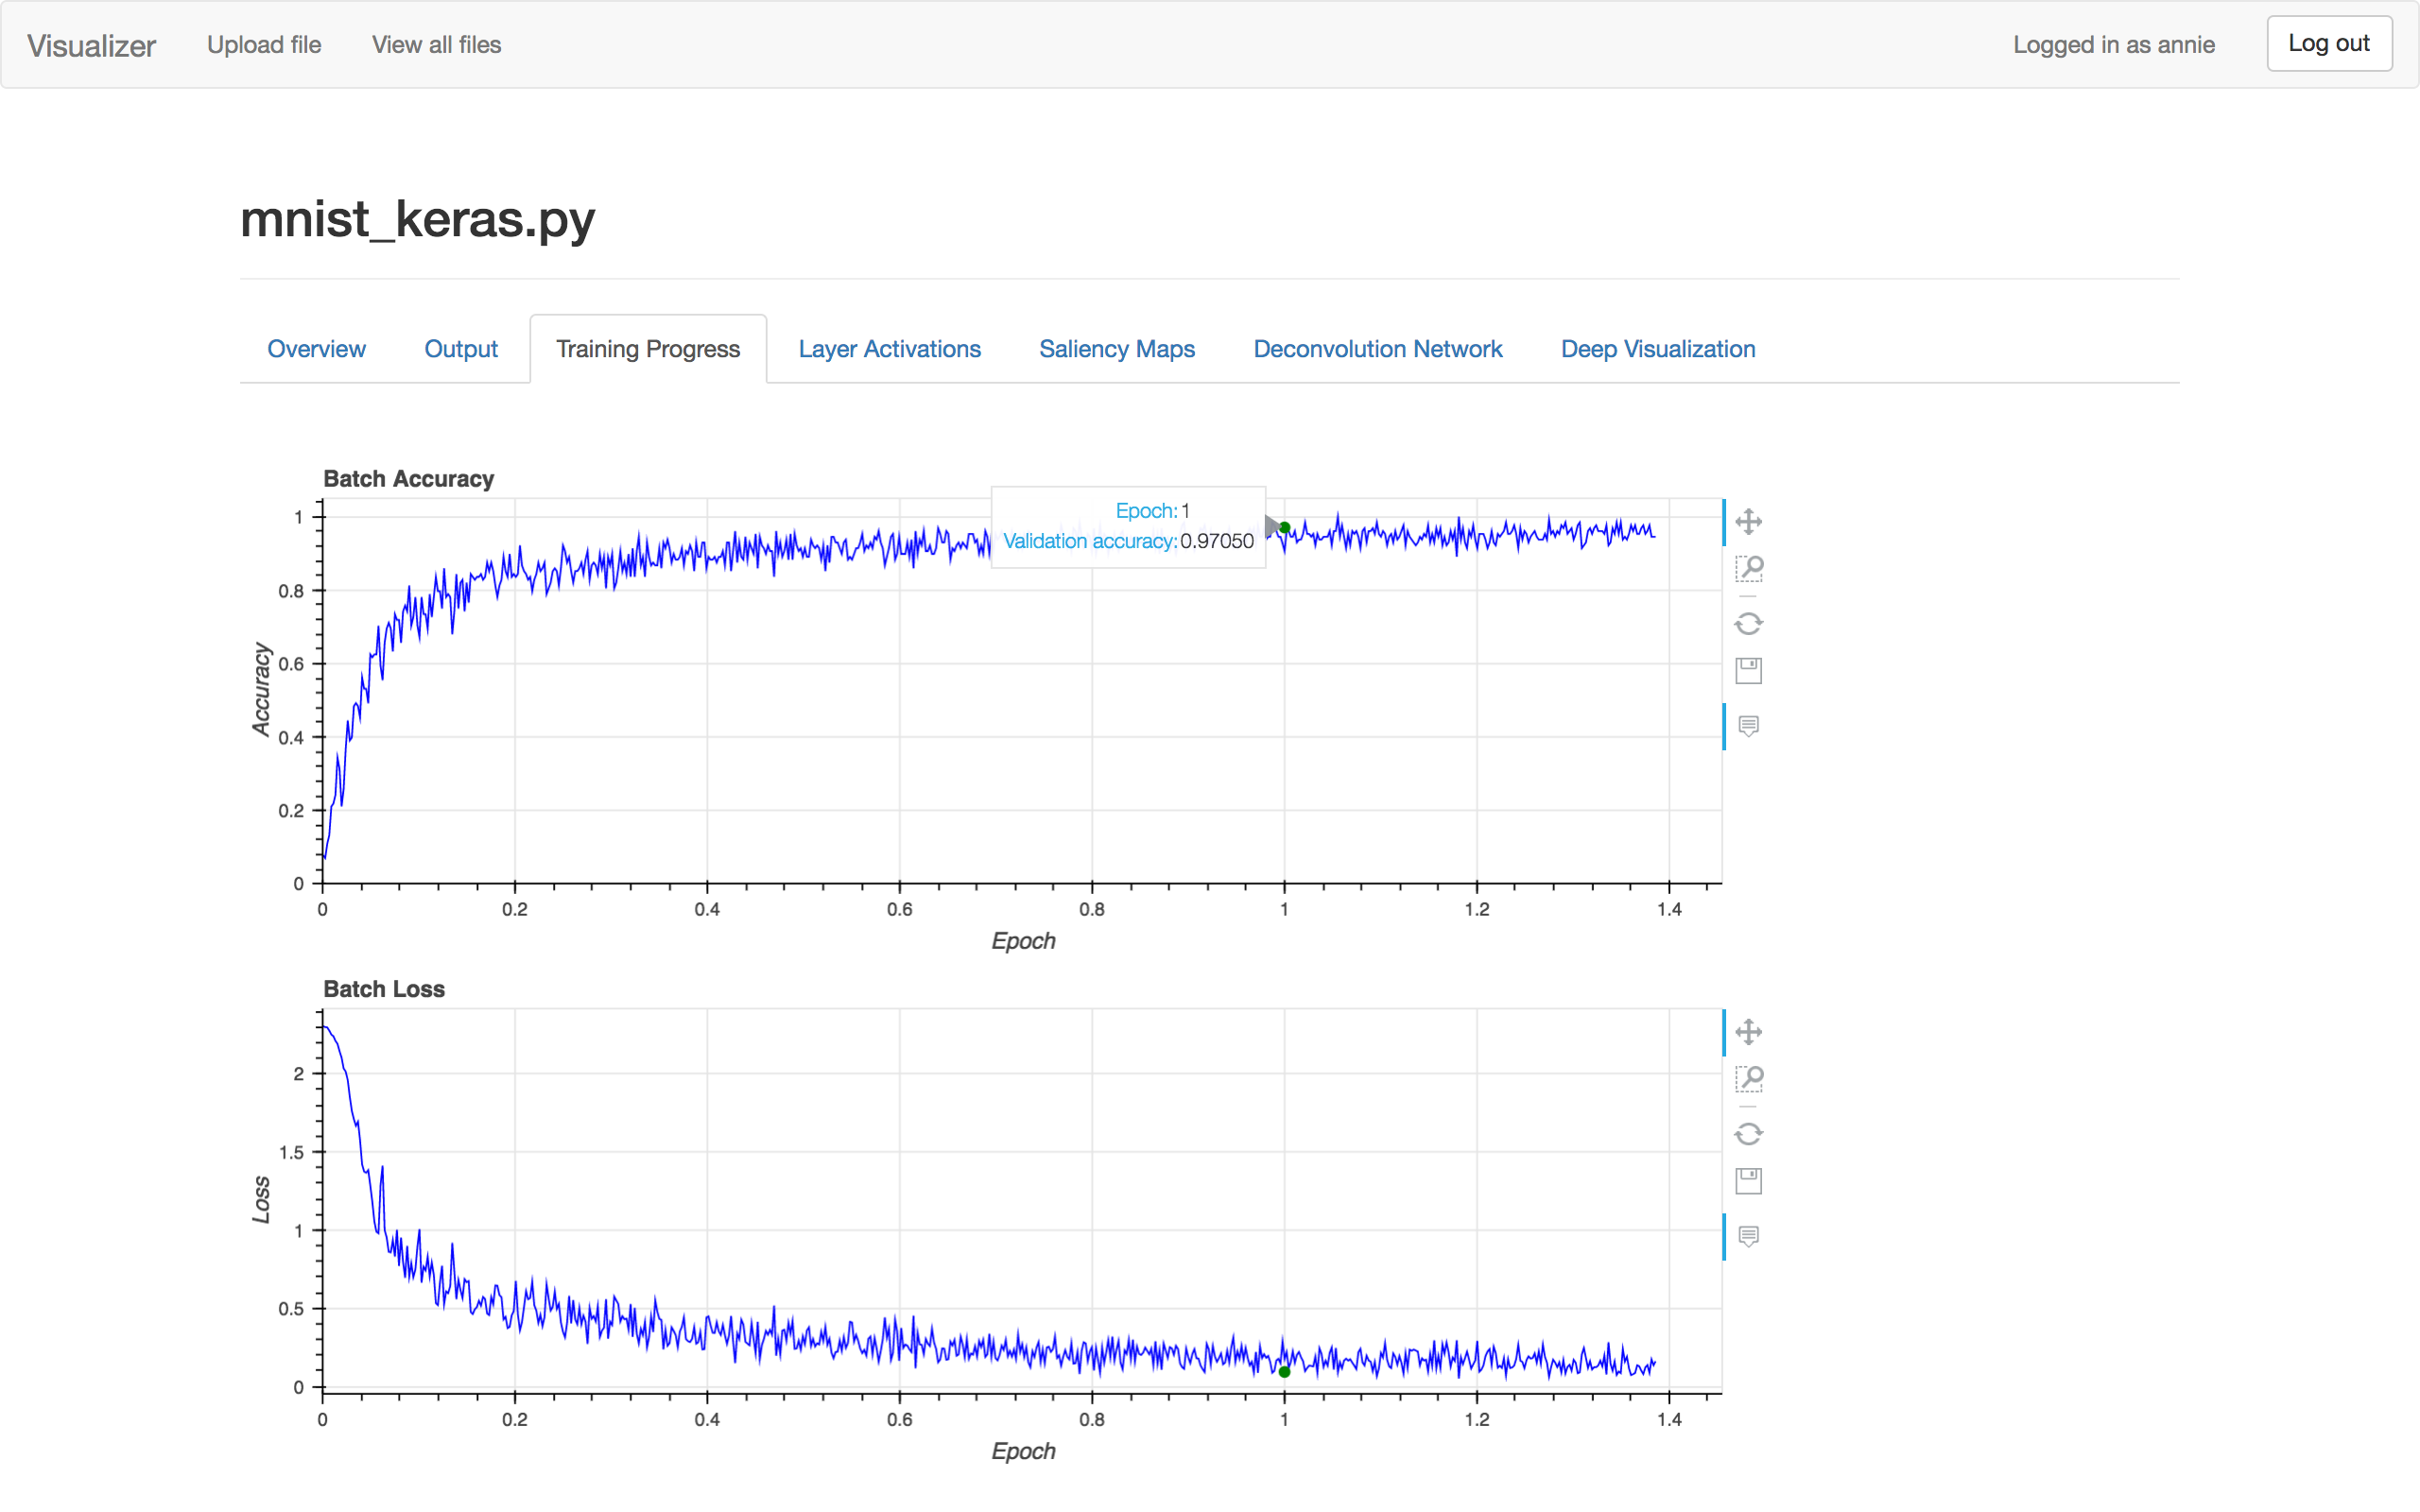
\includegraphics[width=0.8\textwidth]{fig/screenshots/training_prog_val.png}}
        \caption{Training progress}
        \label{trainingprog-tab}
\end{figure}

\noindent \textbf{Note: }The next tabs described require that you have added the corresponding callbacks to your code. \\

\noindent The training progress tab in \textbf{Fig. \ref{trainingprog-tab}} naturally shows the progress of the training. Two plots are available: one for the accuracy and one for the loss. The data shown is the accuracy and loss for each batch in the training (unlike the command line output which shows the average accuracy and loss for the current epoch) over the epoch share. This will give you an overview of how the accuracy and loss are changing through the training process. If you have enabled validation in your Keras code, the validation accuracy and validation loss will be displayed on the graph at each full epoch as a green, circular point. You can hover over these points to see the exact value if you have the hover tool selected on the toolbar. Other tools available are zooming and panning the plot, as well as saving the plot and resetting to the default view. \\

% Layer activations

\begin{figure}[h!]
    \centering
        \frame{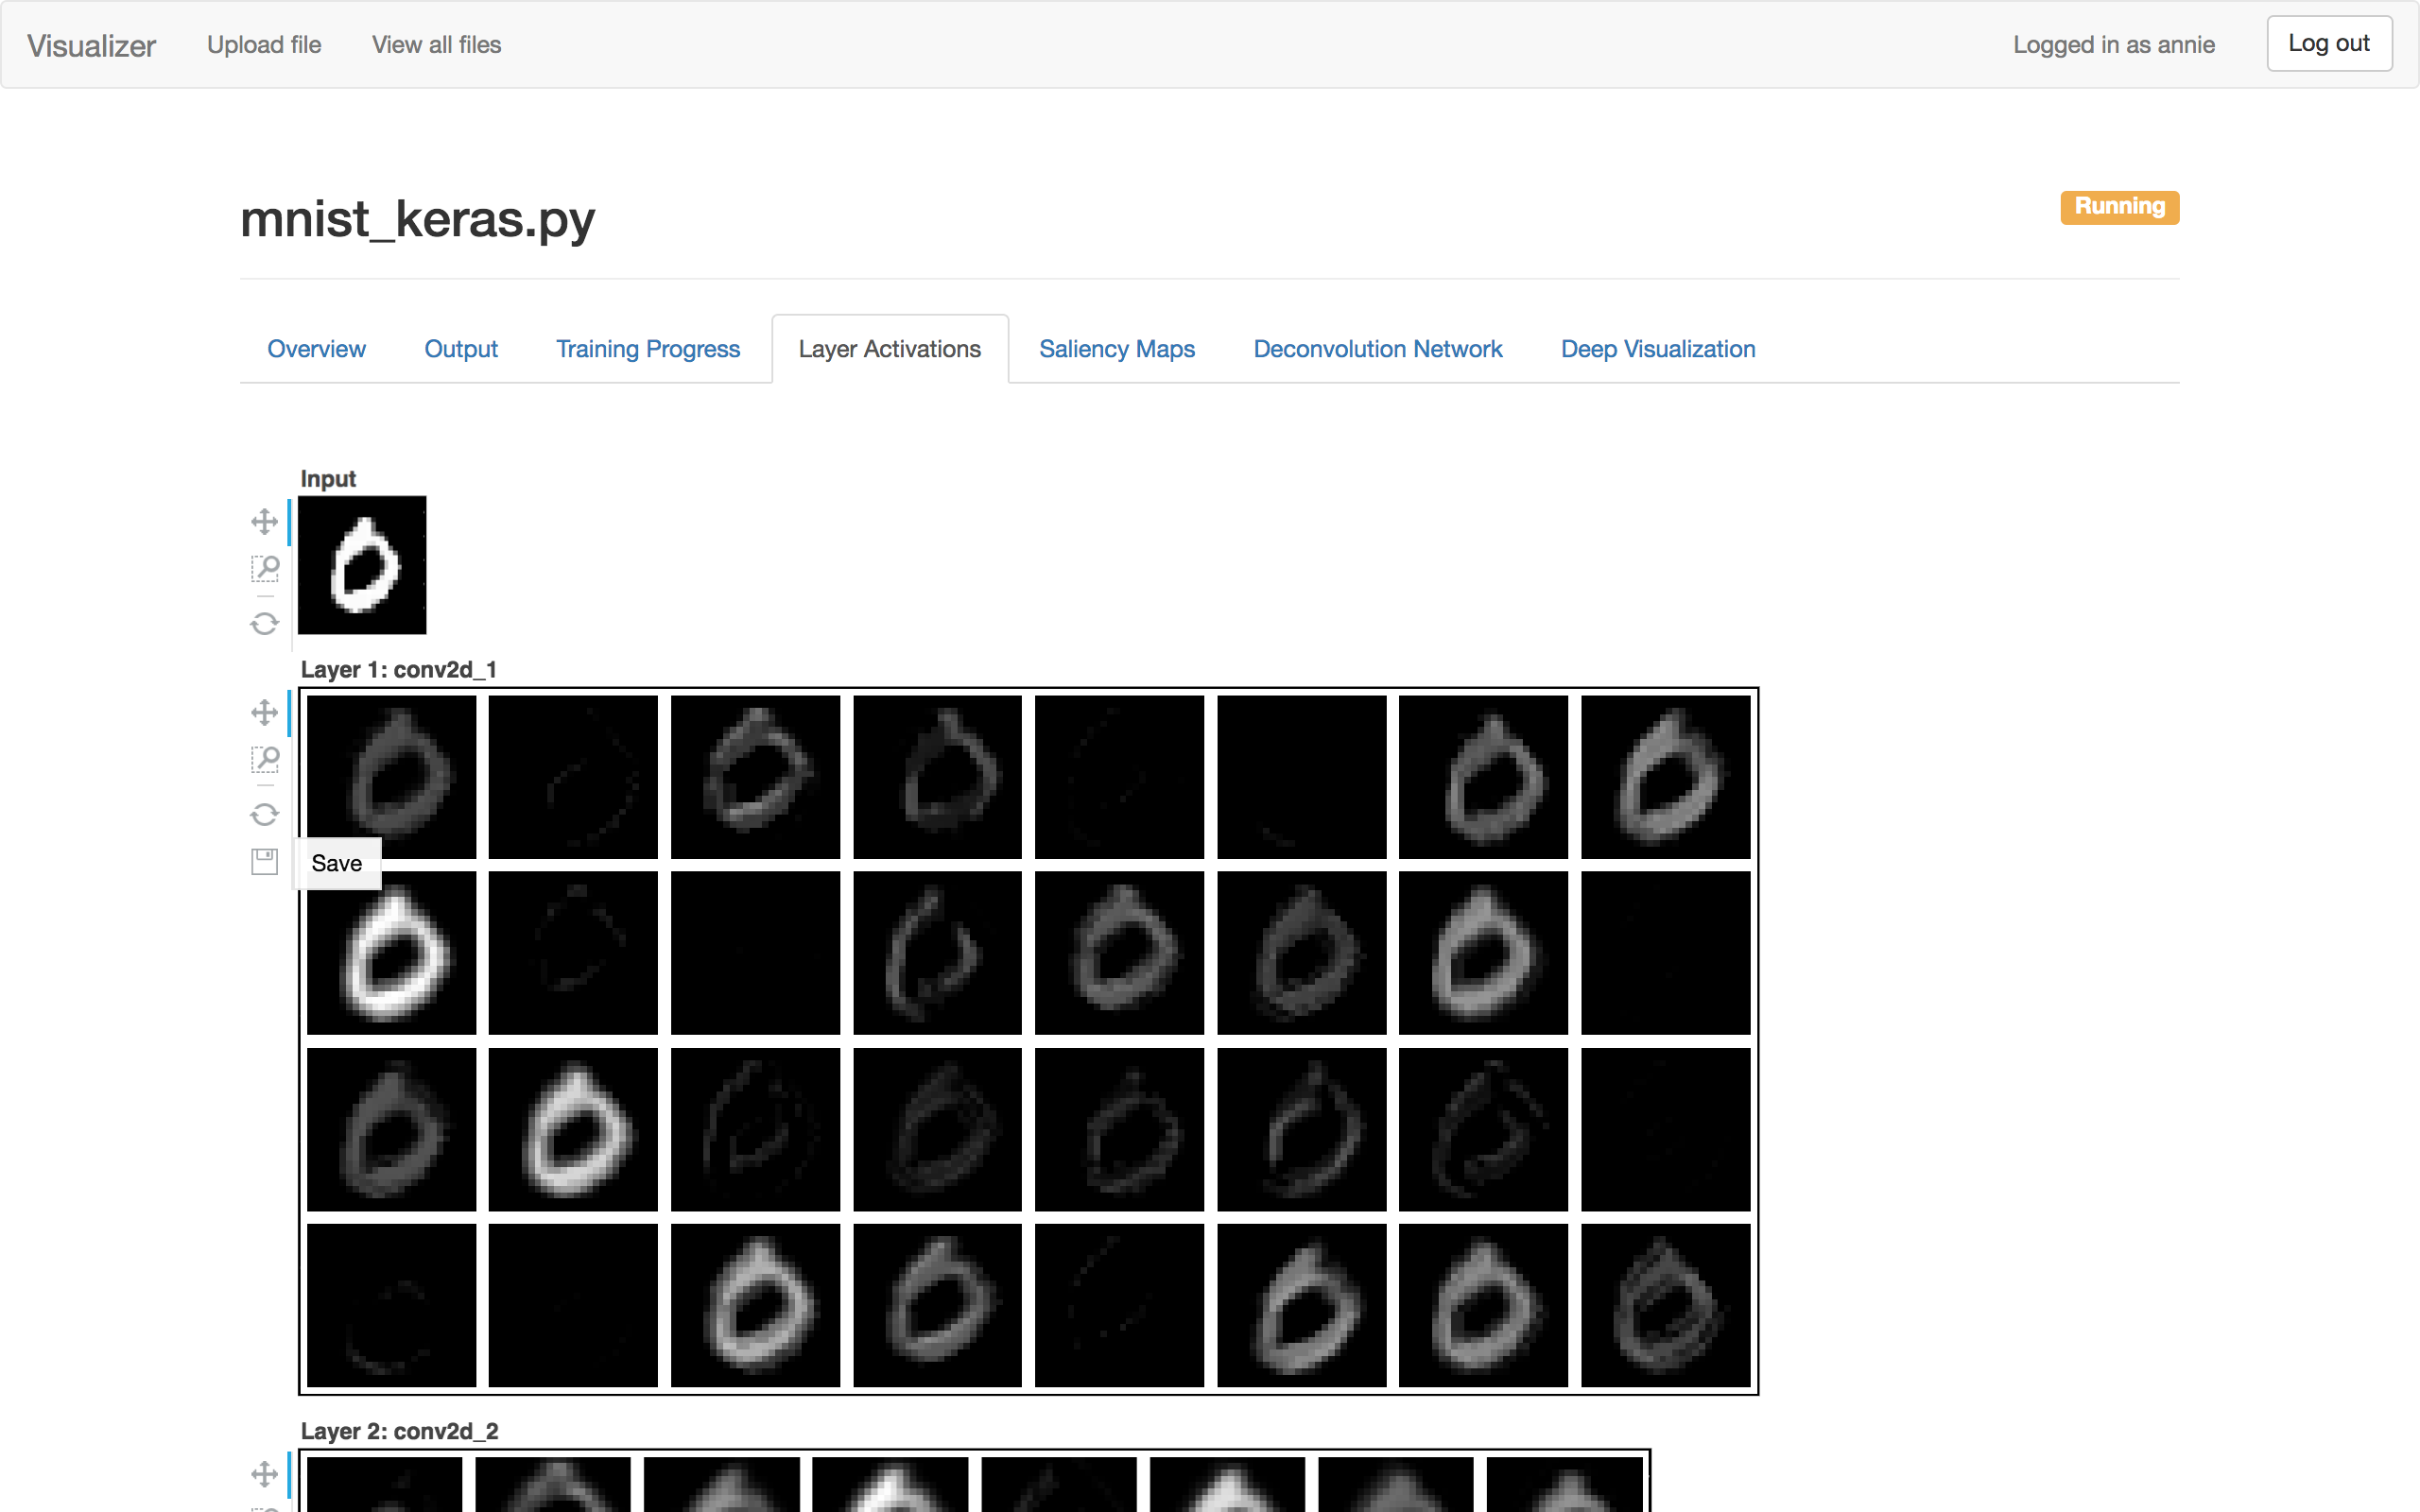
\includegraphics[width=0.8\textwidth]{fig/screenshots/layeract1.png}}
        \caption{Layer activations part 1}
        \label{layeract-tab1}
\end{figure}

\begin{figure}[h!]
    \centering
        \frame{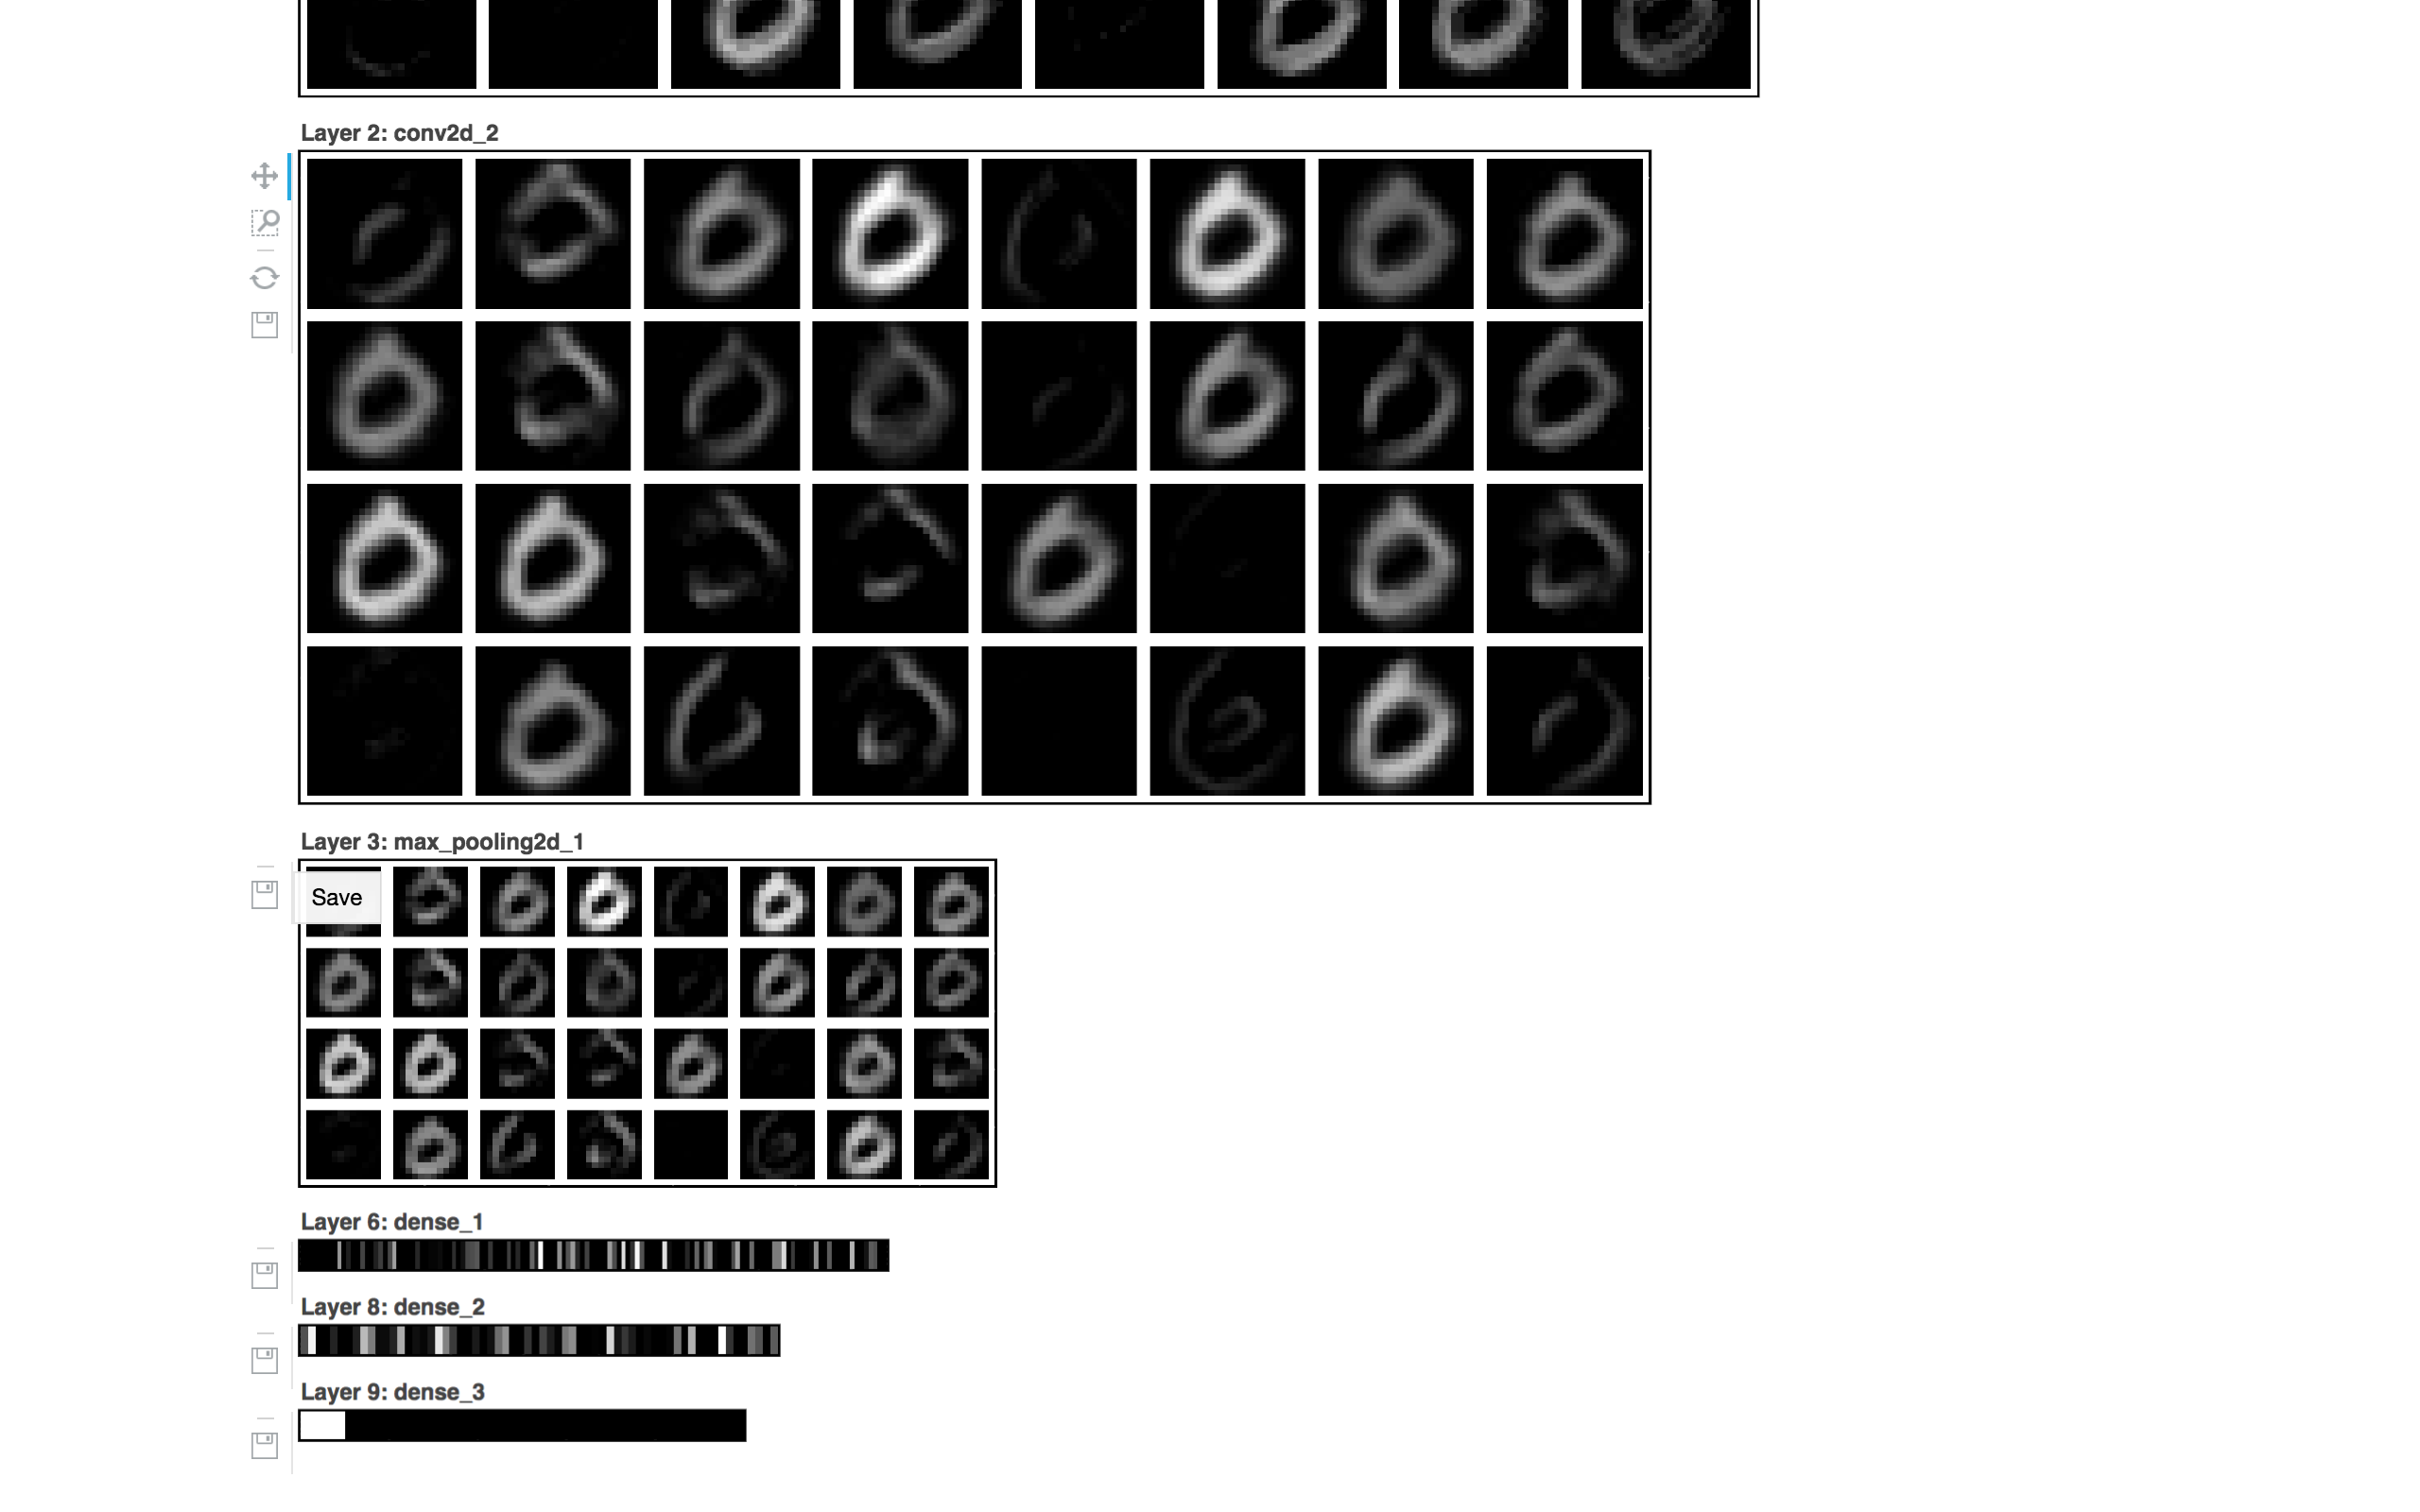
\includegraphics[width=0.8\textwidth]{fig/screenshots/layeract2.png}}
        \caption{Layer activations part 2}
        \label{layeract-tab2}
\end{figure}

\noindent The next tab, seen in \textbf{Fig. \ref{layeract-tab1}} and \textbf{Fig. \ref{layeract-tab2}}, shows the layer activations. Note that this tab may take some time to load, depending on the size of your input image and the number of layers in your network. Once loaded, you can see the input image, followed by the activations for the different layers. Input, dropout and flatten layers are automatically excluded if not specified otherwise in the callback. For layers with 3D output, like convolutional and pooling layers, the activations of the filters are concatenated into grids separated by white borders. Layers with 1D output are also displayed in image format, with each output unit as a pixel. \\

% saliency map

\begin{figure}[h!]
    \centering
        \frame{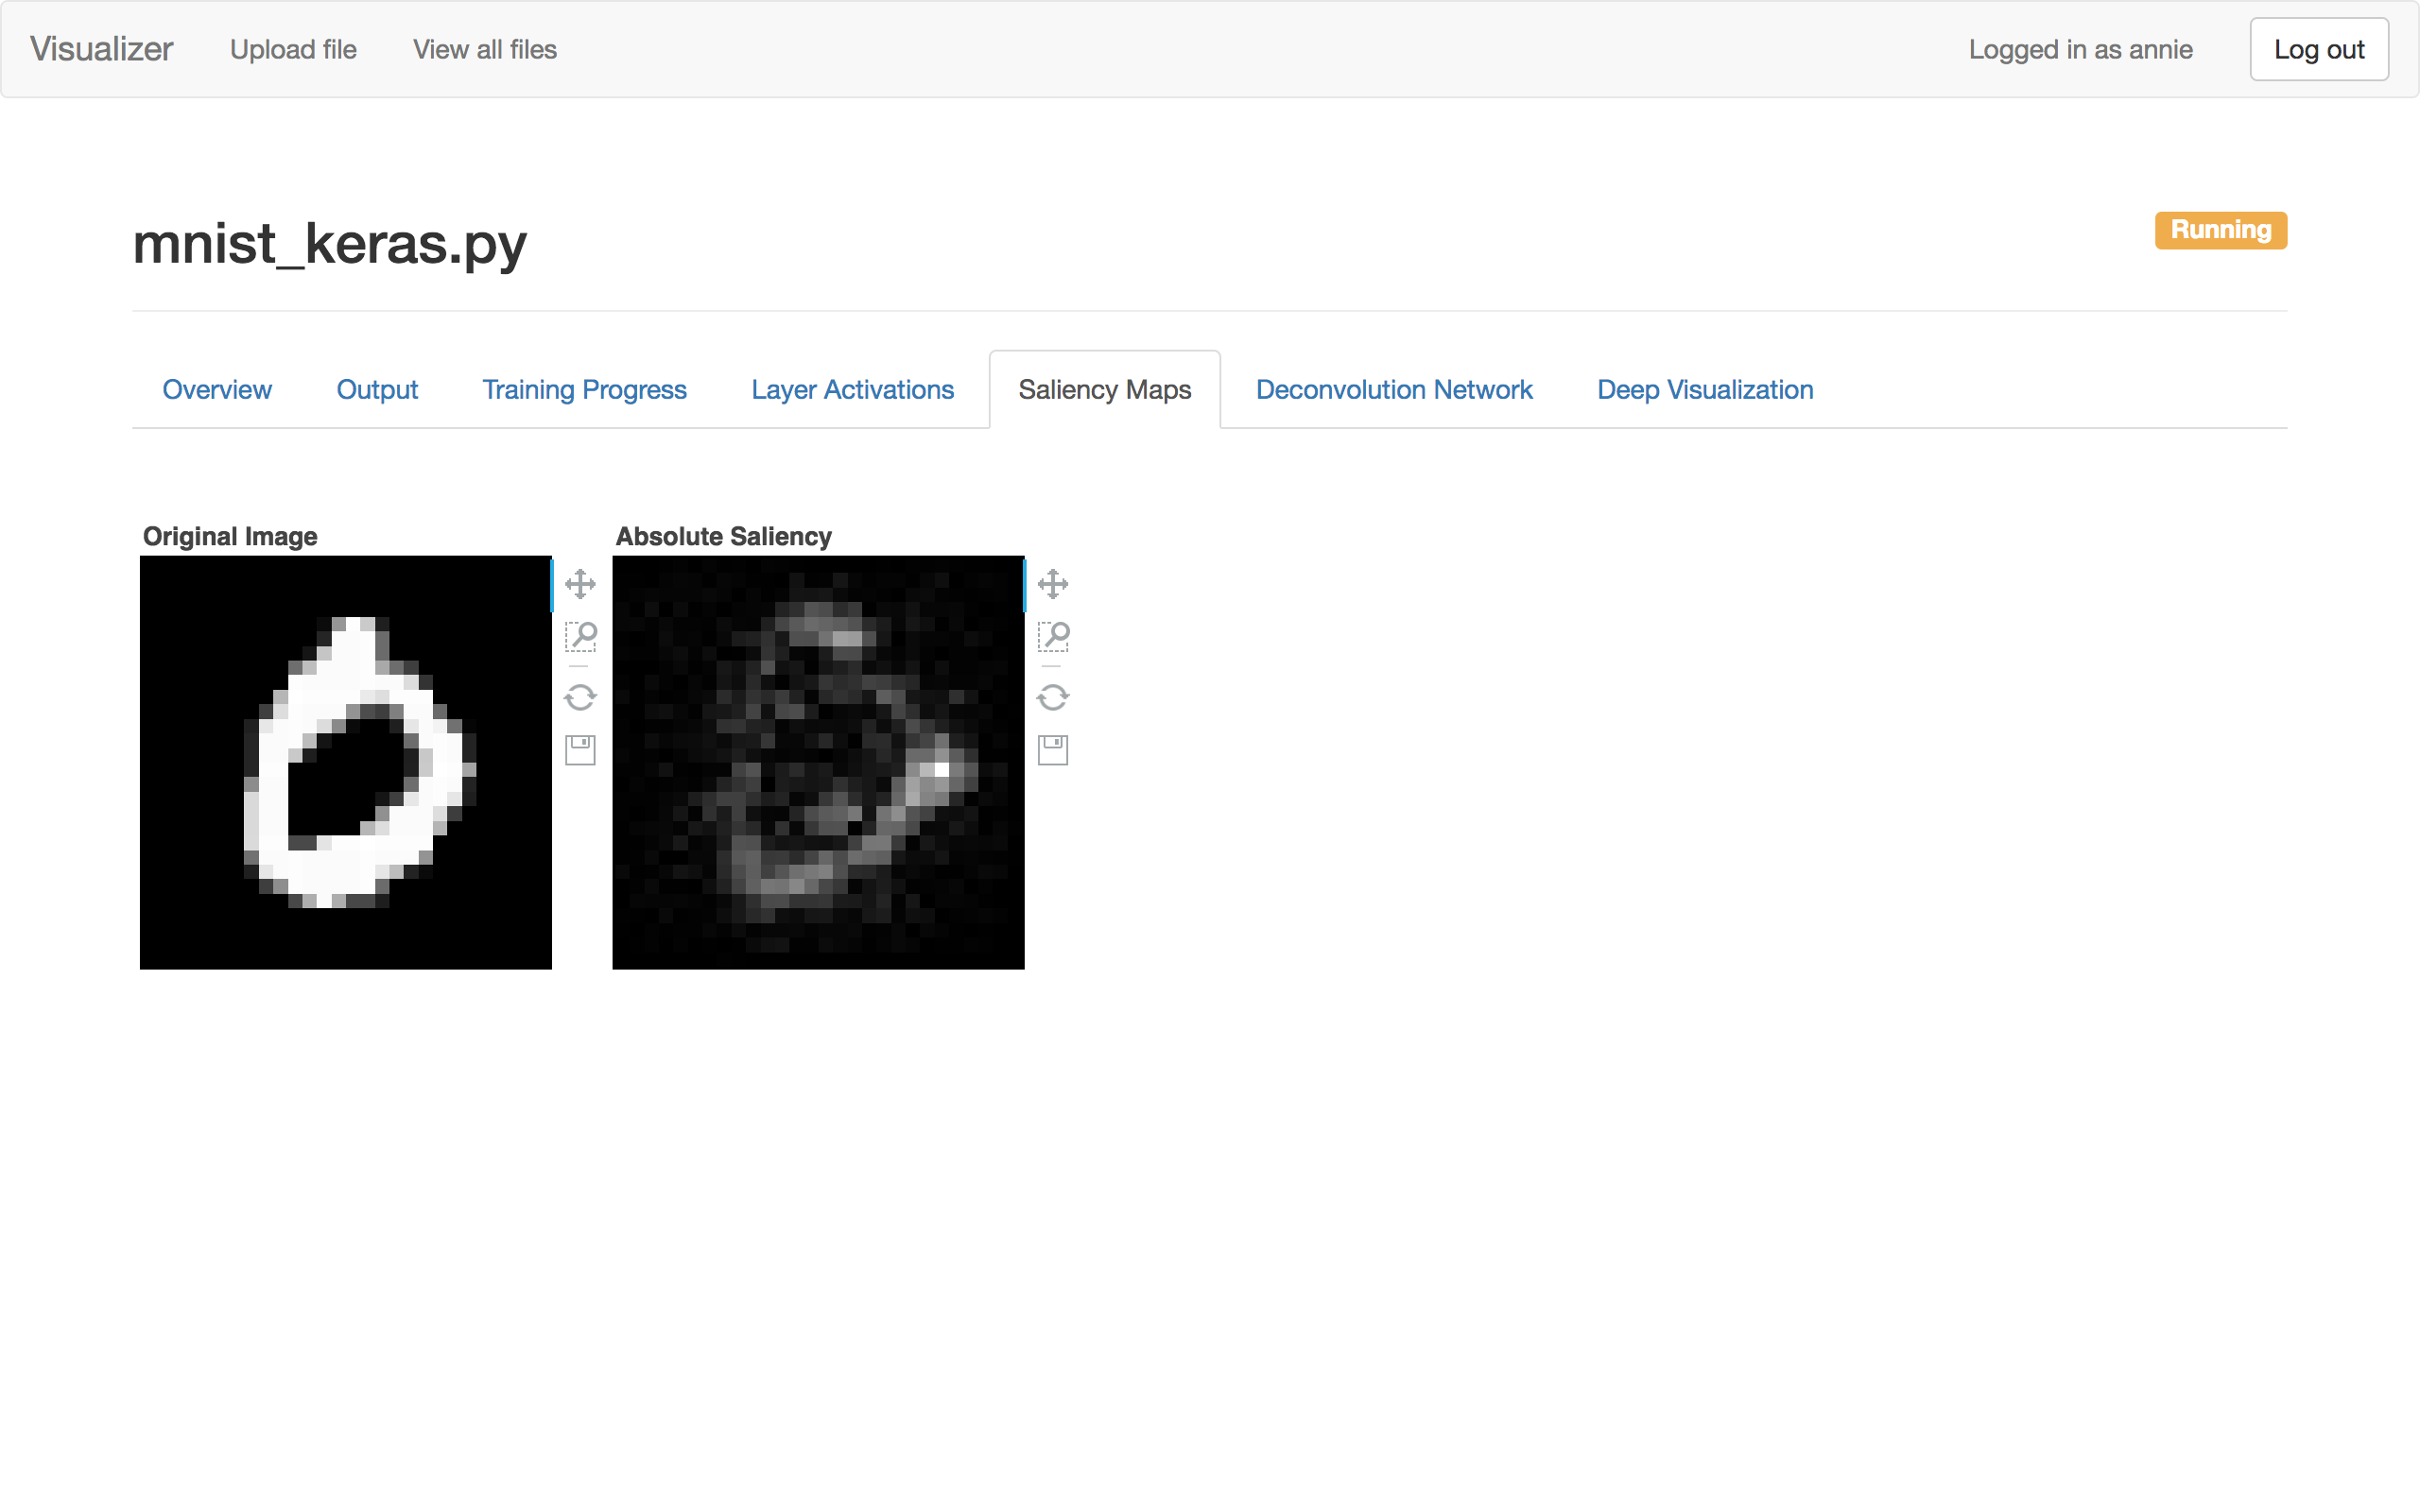
\includegraphics[width=0.8\textwidth]{fig/screenshots/saliencymap.png}}
        \caption{Saliency map}
        \label{saliency-tab}
\end{figure}

\noindent We can view the saliency map of the uploaded visualization image in the next tab, as shown in \textbf{Fig. \ref{saliency-tab}}. The left figure shows the original image, while the right figure shows the computed saliency map. The tools are linked so that if you zoom in on a region of the original image, the same zoomed in region will be displayed in the saliency map, and vice versa. The saliency map indicates to what degree each pixel in the visualization image influences the specific class outcome. The important regions are easily identified by their brightness. The saliency map can help you to see which parts of the visualization image that your network deems more important when deciding upon the classification score chosen.  \\

\begin{figure}[h!]
    \centering
        \frame{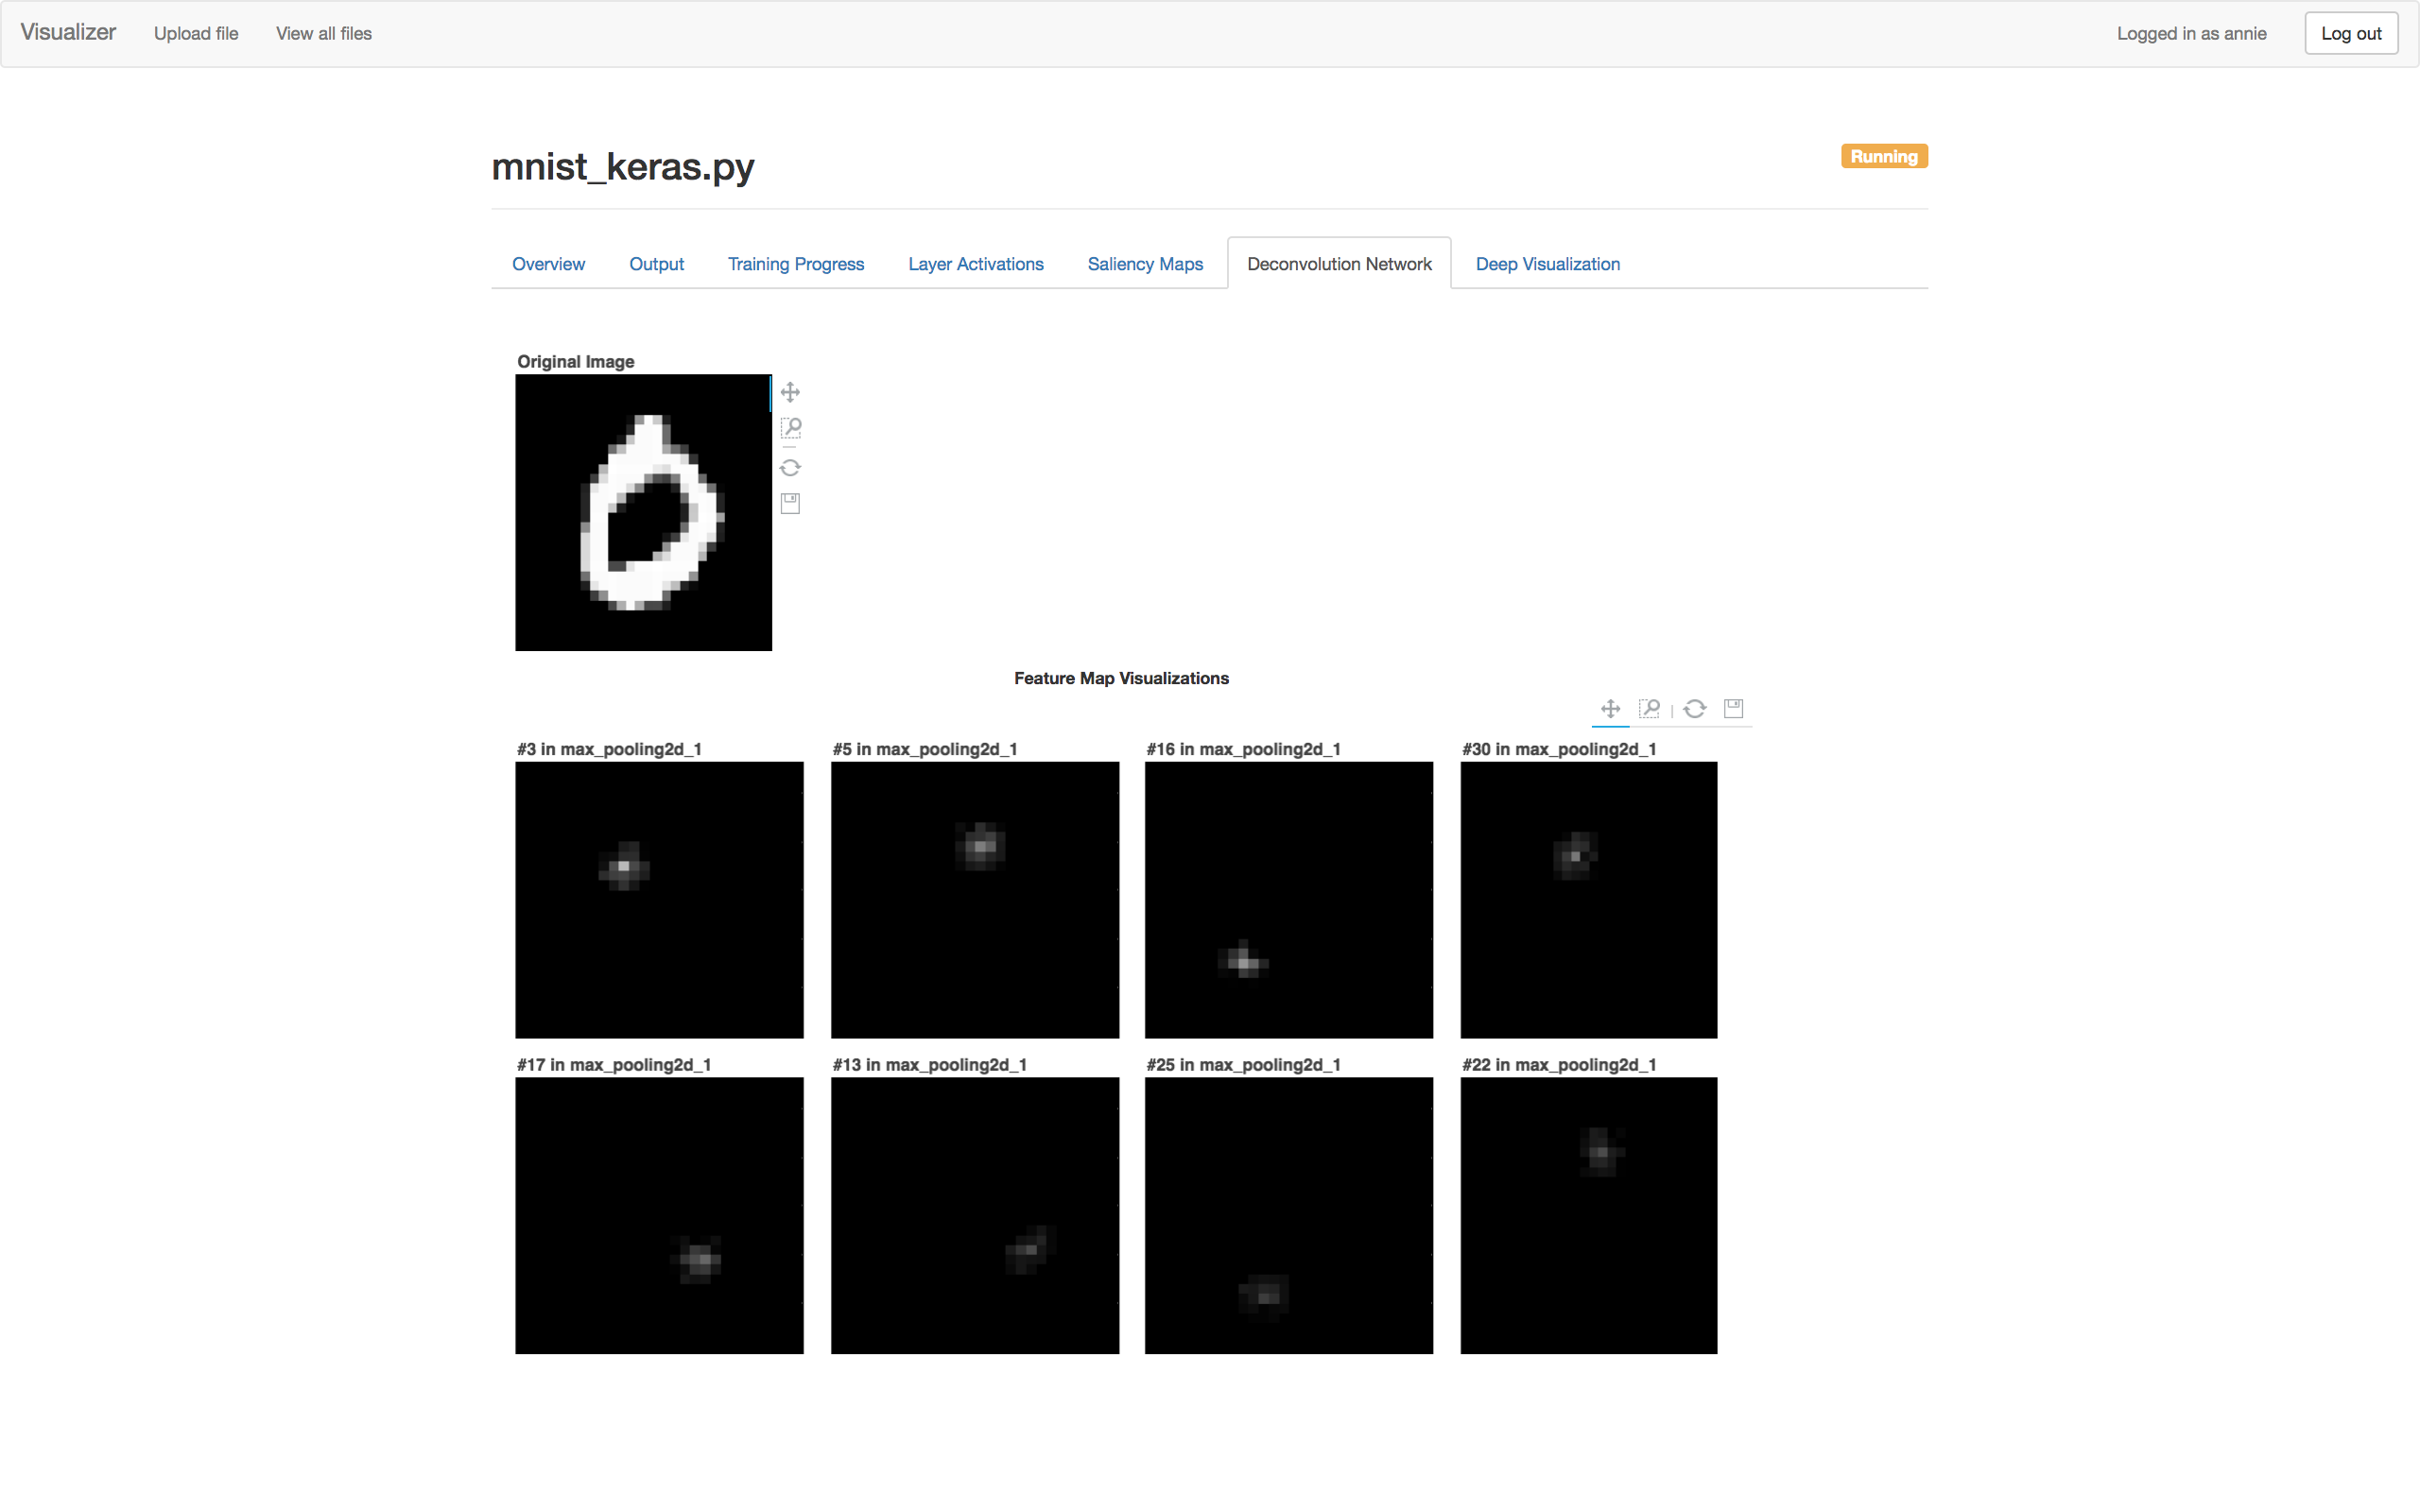
\includegraphics[width=0.8\textwidth]{fig/screenshots/deconv.png}}
        \caption{Deconvolutional network}
        \label{deconv-tab}
\end{figure}

\noindent The next tab shows the deconvolutional network visualization, seen in \textbf{Fig. \ref{deconv-tab}}. The top figure shows the uploaded visualization image. Below the original image, there is a grid of figures showing the reconstructed input based on the feature maps selected for visualization. The visualizations show the pattern in the visualization image that was responsible for eliciting activations in the specific feature map. This pattern can reveal what a certain part of the network finds important and what it is looking for in an image. The tools of the figures are linked together similar to the saliency map figures. Additionally, if you click the save tool, all of the deconvolutional visualizations will be downloaded.\\

\begin{figure}[!h]
    \centering
        \frame{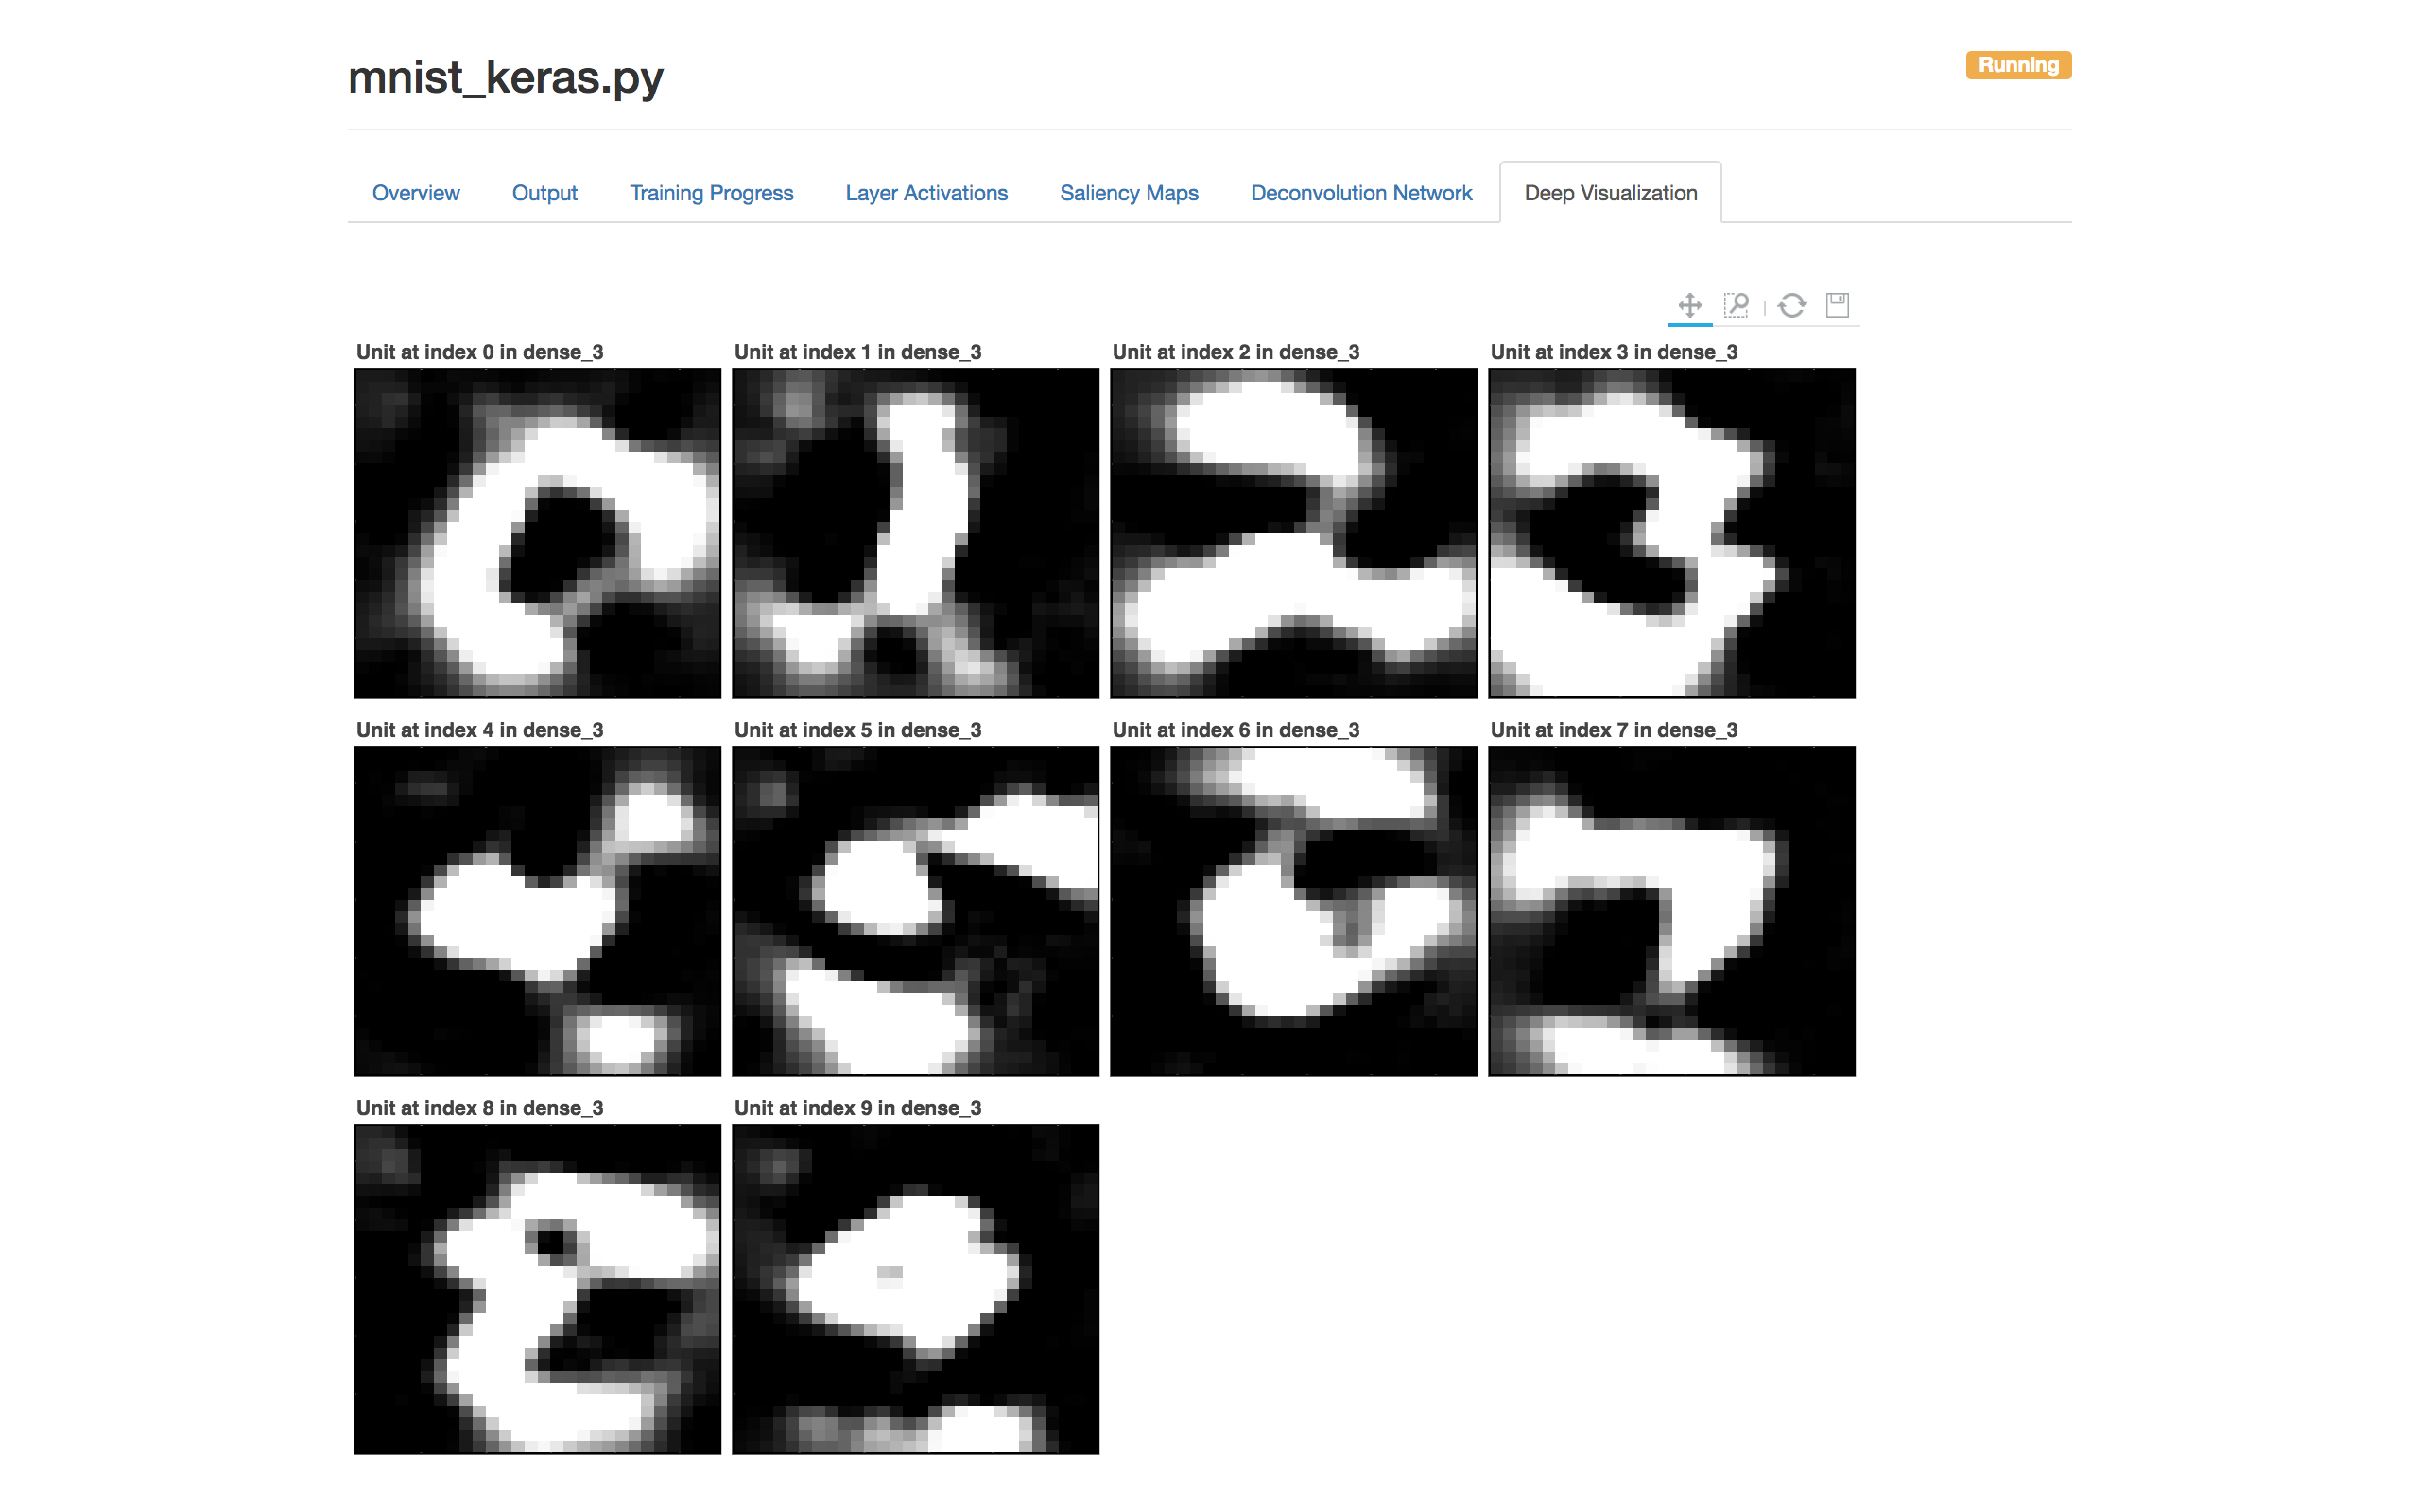
\includegraphics[width=0.8\textwidth]{fig/screenshots/deepvis.png}}
        \caption{Deep visualization}
        \label{deepvis-tab}
\end{figure}

\noindent The final tab, as seen in \textbf{Fig. \ref{deepvis-tab}}, shows the images created using deep visualization. This technique does not utilize the uploaded visualization image. The page presents a grid of figures, with a synthesized image for each network unit chosen for visualization. The synthesized images are optimized to maximally activate their corresponding unit. In other words, they show what the selected units are looking for in an image. \\

\noindent For a more thorough explanation of each visualization technique, visit \autoref{sec:visualization-theory}.

\cleardoublepage